%
% paper.tex -- master LaTeX file for ``ImP: The Image Processing Language''
%
\newcommand{\sys}{CLAM}
\newcommand{\longtitle}{\sys{}: The Concise Linear Algebra Manipulation Language}
\newcommand{\authorlist}{Jeremy Andrus and Robert Martin and Kevin Sun and Yongxu Zhang}
\newcommand{\authoremails}{\{jca2119, rdm2128, kfs2110, yz2419\}@columbia.edu}

% Build Project proposal only (default for now)
\ifcsname ifproposal\endcsname\else
  \expandafter\let\csname ifproposal\expandafter\endcsname
                  \csname iftrue\endcsname
\fi
% Build Language Reference Manual only
\ifcsname ifrefman\endcsname\else
  \expandafter\let\csname ifrefman\expandafter\endcsname
                  \csname iffalse\endcsname
\fi
\ifcsname ifbook\endcsname\else
  \expandafter\let\csname ifbook\expandafter\endcsname
                  \csname iffalse\endcsname
\fi

% Document Class
\ifbook
  \documentclass[10pt,letterpaper,titlepage,onecolumn,oneside]{book}
\else
  \documentclass[10pt,letterpaper,onecolumn,oneside]{article}
\fi

\usepackage[margin=1.0in]{geometry}
\usepackage[utf8x]{inputenc}
\usepackage{ucs}
\usepackage{amsmath}
\usepackage{amsfonts}
\usepackage{amssymb}
\usepackage[usenames,dvipsnames]{color}
\usepackage{listings}
\usepackage{graphicx}
\usepackage{underscore}
% hyphenat redefines "BreakableUnderscore", so I need
% to do some LaTeX gymnastics to make it work...
\makeatletter
\let\BreakableUnderscore\@undefined
\makeatother
\usepackage{hyphenat}
\usepackage{lastpage}
\usepackage{balance}
\usepackage{cite}
\usepackage{pdfsync}
\usepackage[colorlinks=false,
    pdftitle={\longtitle{}},
    pdfborder={0 0 0},
    pdfauthor={\authorlist{}},
    pdfdisplaydoctitle=true,
    plainpages=false]{hyperref}
\usepackage{breakurl}

\setlength{\parindent}{0in}
\addtolength{\parskip}{\baselineskip}

% other useful commands
\newcommand{\comment}[1]{}

\begin{document}

% this usually saves about a line-or-two by squeezing inter-sentence space
%\frenchspacing

\title{\longtitle{}}
\author{\authorlist{}\\\authoremails{}\\\\Columbia University\\COMS W4115: Programming Languages and Translators}
\maketitle

% Body of the paper in different files
\ifproposal
  % Project Proposal
  \section*{Language Proposal}

\definecolor{DarkBlue}{rgb}{0.0, 0.08, 0.65}
\definecolor{DarkRed}{rgb}{0.65, 0.08, 0.0}
\definecolor{DarkGreen}{rgb}{0.08, 0.35, 0.08}
\definecolor{Grey}{rgb}{0.55, 0.55, 0.55}
\definecolor{Yellow}{cmyk}{0.0, 0.08, 0.5, 0.3}
\definecolor{Brown}{rgb}{0.55, 0.27, 0.08}
\definecolor{LightBlue}{cmyk}{0.8, 0.1, 0.0, 0.1}
\lstdefinelanguage{PLTF11}{
    classoffset=0,
	morekeywords={somethingsomethingsomething},
    keywordstyle={\color{Yellow}\itshape\bfseries},
    classoffset=1,
    morekeywords={Uint8,Uint16,Uint32,Int8,Int16,Int32,Angle,Matrix,Image,Kernel},
    keywordstyle={\color{DarkBlue}\bfseries},
    classoffset=2,
	morekeywords={imgread,imgwrite},
	keywordstyle={\color{Brown}},
	otherkeywords={:=,**,=,|,:},
	moredelim=*[s][\color{LightBlue}]{\#[}{]},
	moredelim=*[s][\color{DarkGreen}\itshape]{\$(}{)},
    morecomment=[l]{//},
    commentstyle={\color{Grey}\bfseries},
    morestring=[b]",
    stringstyle={\color{DarkRed}},
    sensitive=true,
}

\comment{
Possible language names:
LIP - Linear Image Processing (+1)
MILA - Manipulate Images w/ Linear Algebra
CLAM - Color & Light Algebraic Manipulation/Convolutions, Linear Algebra & Matrices
GeBR - Middle part of "alGeBRa", and a rearrangement of RGB - because it manipulates colors.
}

\sys{} is a linear algebra manipulation language specifically targeted for
image processing. It provides an efficient way to express complex image
manipulation algorithms through compact matrix operations. Traditional image
processing is performed using a language such as C, or C++. Algorithms in these
languages are quite complex and error-prone due to the large number of lines of
code required to implement something as conceptually simple as, "make this image
blurry." The complexity arises from the need to perform elaborate calculations
on every pixel in an image. For example, to blur an image you first need to
calculate the luminance of the pixel (from the red, green, and blue channels),
then you need to mathematically combine this with the luminance of adjacent pixels,
and finally re-calculate red, green, and blue values for an output image.

\sys{} will simplify image processing, and more generally linear algebra, through
domain-specific data types and operators. The basic data type in \sys{} is a 
\texttt{Matrix}. Matrices can be manipulated by operators that perform functions
such as matrix multiplication, or rotation. An \texttt{Image} is another \sys{}
data type which is expressed as a collection of matrices, or channels. For example,
when reading an image into memory, \sys{} creates a \emph{Red}, \emph{Green}, and
\emph{Blue} channel automatically. Additional Image channels can either be assigned,
or calculated using an expression syntax which defines a calculation involving the
values of other, previously defined, channels. The basic image processing operator
in \sys{} is the convolution operator. This operator takes a channel and a
\texttt{Kernel}, another basic data type, and outputs an \texttt{Image}. This
operator convolves each \texttt{Matrix} within the \texttt{Kernel} with the input channel,
and collects the resulting output channels into an \texttt{Image}.

Two primary use cases of \sys{} are basic image information extraction, and
filtering. The compact syntax and powerful basic data types of \sys{} will make
information extraction, such as finding all the edges in an image, simple, compact,
and easy to read.

\subsection*{Features}
\sys{} uses implicit loops, i.e. there is no explicit looping construct in the
language. Loops are implicitly defined by per-pixel matrix or convolution
operations. Additionally, \sys{} automatically determines or calculates image and matrix
dimensions. There is no need to explicitly size these data types. This further
reduces complexity, and eliminates frequent mistakes such as going beyond array
bounds in a calculation.

\subsection*{Example Syntax}

The goal of the \sys{} syntax will be to make conceptually simple image
manipulations into simple language constructs. For instance, convolutions make
frequent use of constant matrices, so our language will provide a simple way
to specify them, such as:
\begin{lstlisting}[language=PLTF11]
    Matrix sobelGy := { +1 +2 +1 |  0  0  0 | -1 -2 -1 };
\end{lstlisting}

Another common image processing technique is performing the same calculation
on every pixel in the image. An example of this is calculating the luminance
of a pixel from the red, green, and blue channels. \sys{} makes this calculation
simple and compact by defining an additional image channel. Assuming there exists
an instance of a \texttt{Image} variable named, \emph{myimg}, a channel can be
added to the image with:
\begin{lstlisting}[language=PLTF11]
    Int32 myimg:Luminance := #[ (3*Red + 6*Green + 1*Blue) / 10 ];
\end{lstlisting}
Where the expression within \texttt{\#[ \ldots ]} is evaluated once for every
pixel in the \texttt{Image}. The \emph{Red}, \emph{Green}, and \emph{Blue} variables
correspond to previously defined channels in \emph{myimg}, and their values during
expression evaluation will be the value of the corresponding channel at the current
pixel location.

Image processing also frequently involves describing a series of operations that
should be carried out for each pixel, and then repeating it for every pixel in an
image. \sys{} makes it simple to describe this process through the \texttt{Kernel}
data type and the convolution operator. Here is an example of how one might perform
a Sobel edge detector in the \sys{} language:
\lstinputlisting[language=PLTF11,numbers=left,frame=single]{src/sobel.imp}

\else
  
\definecolor{clamLightBlue}{cmyk}{0.8, 0.1, 0.0, 0.1}
\definecolor{clamDarkBlue}{rgb}{0.0, 0.08, 0.65}
\definecolor{clamDarkRed}{rgb}{0.65, 0.08, 0.0}
\definecolor{clamDarkGreen}{rgb}{0.08, 0.35, 0.08}
\definecolor{clamYellow}{cmyk}{0.0, 0.08, 0.5, 0.3}
\definecolor{clamPurple}{rgb}{0.58, 0.0, 0.83}
\definecolor{clamBrown}{rgb}{0.55, 0.27, 0.08}
\definecolor{clamGrey}{rgb}{0.55, 0.55, 0.55}
\lstdefinelanguage{CLAM}{
    classoffset=0,
    keywordstyle={\color{clamYellow}\bfseries}, % default style (used by 'otherkeywords')
    morekeywords={somethingsomethingsomething},
    classoffset=1,
    morekeywords={Uint8,Uint16,Uint32,Int8,Int16,Int32,Calc,Angle,Image,Kernel},
    keywordstyle={\color{clamDarkRed}\bfseries},
    classoffset=2,
    morekeywords={imgread,imgwrite},
    keywordstyle={\color{clamPurple}\bfseries},
    classoffset=3,
    otherkeywords={=,|,\,,:,:=,**,@},
    morecomment=[l]{//},
    morecomment=[n]{/*}{*/},
    commentstyle={\color{clamGrey}\bfseries},
    morestring=[b]",
    stringstyle={\color{clamBrown}},
    moredelim=*[s][\color{clamLightBlue}]{\#[}{]\#},
    moredelim=*[s][\color{clamBrown}]{[}{]},
    moredelim=*[s][\color{clamDarkGreen}]{\{}{\};},
    sensitive=true,
    showstringspaces=false,
    showspaces=false,
    showtabs=false,
    frame=single,
    numbers=left,
    basicstyle=\ttfamily,
}


  % Adapted from vim Ocaml syntax highlighting

\definecolor{ocamlLightBlue}{cmyk}{0.8, 0.1, 0.0, 0.1}
\definecolor{ocamlDarkBlue}{rgb}{0.0, 0.08, 0.65}
\definecolor{ocamlDarkRed}{rgb}{0.65, 0.08, 0.0}
\definecolor{ocamlDarkGreen}{rgb}{0.08, 0.35, 0.08}
\definecolor{ocamlYellow}{cmyk}{0.0, 0.08, 0.5, 0.3}
\definecolor{ocamlPurple}{rgb}{0.58, 0.0, 0.83}
\definecolor{ocamlBrown}{rgb}{0.55, 0.27, 0.08}
\definecolor{ocamlGrey}{rgb}{0.55, 0.55, 0.55}
\lstdefinelanguage{OCaml}{
    classoffset=0,
    keywordstyle={\color{ocamlPurple}\bfseries},
    morekeywords={somethingsomethingsomething},
    classoffset=1,
    morekeywords={and,as,assert,class,constraint,else,exception,external,fun,function,in,inherit,initializer,land,lazy,let,match,method,module,mutable,new,of,open,parser,private,raise,rec,then,try,type,val,virtual,when,while,with,do,value},
    keywordstyle={\color{ocamlDarkRed}\bfseries},
    classoffset=2,
    morekeywords={true,false,array,bool,char,exn,float,format,format64,int,int32,int64,lazy\_t,list,nativeint,option,string,uint},
    keywordstyle={\color{ocamlDarkBlue}\bfseries},
    classoffset=3,
    morekeywords={StringMap,String,List,Printf,Lexing,Scanner,Map,Make,Pervasives,Failure,VarMap,Parser,Ast},
    keywordstyle={\color{ocamlDarkGreen}},
    classoffset=4,
    otherkeywords={asr,lor,lsl,lsr,lxor,mod,not,::,;,|,@,->,<-,[],:=,;;,^,&&},
    morecomment=[l]{//},
    morecomment=[n]{(*}{*)},
    commentstyle={\color{ocamlGrey}\bfseries},
    morestring=[b]",
    stringstyle={\color{ocamlBrown}},
    moredelim=*[s][\color{ocamlBrown}]{'}{'},
    sensitive=true,
    showstringspaces=false,
    showspaces=false,
    showtabs=false,
    numbers=left,
    frame=single,
    breaklines=true,
    basicstyle=\ttfamily\scriptsize,
}


  \ifrefman
    % Language Reference Manual
    \section*{Language Reference Manual}
    Our language reference manual goes here.
Probably should cite the K\&R C reference manual~\cite{DBLP:books/ph/KernighanR88} here.

    \clearpage
  \else
    % Final Project report is the default output here
    \tableofcontents
    \chapter{Introduction}

\sys{} is a linear algebra manipulation language specifically targeted for
image processing. It provides an efficient way to express complex image
manipulation algorithms through compact matrix operations. Traditional image
processing is performed using a language such as C, or C++. Algorithms in these
languages are quite complex and error-prone due to the large number of lines of
code required to implement something as conceptually simple as, "make this image
blurry." The complexity arises from the need to perform elaborate calculations
on every pixel in an image. For example, to blur an image you first need to
calculate the luminance of the pixel (from the red, green, and blue channels),
then you need to mathematically combine this with the luminance of adjacent pixels,
and finally re-calculate red, green, and blue values for an output image.

\sys{} will simplify image processing, and more generally linear algebra, through
domain-specific data types and operators. The basic data type in \sys{} is a 
\texttt{Matrix}. Matrices can be manipulated by operators that perform functions
such as matrix multiplication, or rotation. An \texttt{Image} is another \sys{}
data type which is expressed as a collection of matrices, or channels. For example,
when reading an image into memory, \sys{} creates a \emph{Red}, \emph{Green}, and
\emph{Blue} channel automatically. Additional Image channels can either be assigned,
or calculated using an expression syntax which defines a calculation involving the
values of other, previously defined, channels. The basic image processing operator
in \sys{} is the convolution operator. This operator takes a channel and a
\texttt{Kernel}, another basic data type, and outputs an \texttt{Image}. This
operator convolves each \texttt{Matrix} within the \texttt{Kernel} with the input channel,
and collects the resulting output channels into an \texttt{Image}.

Two primary use cases of \sys{} are basic image information extraction, and
filtering. The compact syntax and powerful basic data types of \sys{} will make
information extraction, such as finding all the edges in an image, simple, compact,
and easy to read.


    \chapter{Language Tutorial}

\section{Input and Output}

\sys{}'s basic I/O operators are \texttt{imgread} and \texttt{imgwrite}, and every program
will have to call them at least once each to do anything useful. \texttt{imgread}
takes a filename (or integer, see below) as its sole argument and returns an \texttt{Image}.
\texttt{imgwrite} take an \texttt{Image}, a format, and filename (or integer).

\subsection{Your first program}

Using only I/O operators, you can already write a simple program that copies an image from
one location to another. Or, if the output is in a different format than the input,
you have a simple image converter. In either case, you only need two lines of code!

\begin{lstlisting}[language=CLAM,escapechar=\%]
Image input = imgread("source.jpg");
imgwrite(input, "png", "dest.png");
\end{lstlisting}
\ldots or 1 if you're tricky
\begin{lstlisting}[language=CLAM,escapechar=\%]
imgwrite(imgread("source.jpg"), "png", "dest.png");
\end{lstlisting}

\subsection{Using command-line arguments}

This program only copies from \texttt{"source.jpg"} to \texttt{"dest.png"} which is not
very useful.
You'd need to edit the code and recompile to change the source and destination.
To avoid this problem, \texttt{imgread} and \texttt{imgwrite} can both be called with integers
which refer to items in the command-line argument list, giving your code much greater
flexibility. (\sys{} will automatically enforce the correct number of command-line arguments.)

\begin{lstlisting}[language=CLAM,escapechar=\%]
imgread(1); /* Get filename from argv[1]*/
imgwrite(input, "png", 2); /* Get filename from argv[2]*/
\end{lstlisting}

\section{Compiling and Running Your Program}

In order to generate binaries from your \sys{} program, you will need the \texttt{g++} compiler
installed and available in your default \texttt{PATH}. This is because \sys{} uses C/C++ as its
compile target, and leverages existing C/C++ compilers to generate and optimize machine-dependent code.
You can compile your clam program by simply passing your file to \texttt{clam} as the sole argument.
This will automatically output a binary to \texttt{a.out}. You can also specify the name of
the binary with the \texttt{-o} flag, and pass in the source file path with \texttt{-i}.
For example:
\begin{itemize}
  \item \texttt{./clam prog1.clam}
  \item \texttt{./a.out source.jpg dest.png}
  \item \texttt{./clam -i prog1.clam -o copyimg}
  \item \texttt{./copyimg source.jpg dest.png}
\end{itemize}

The full set of options to the \sys{} compiler can be found using the \emph{--help} option, and is
reproduced below:
\begin{lstlisting}[language=make,basicstyle=\ttfamily]
CLAM v0.1
Usage: clam {options} [{<} inputfile]
Options are:
  -o <filename> Specify the output file
  -i <filename> Specify the input file
  -c            Output generated C only
  -t            Print AST debugging information
  -help         Display this list of options
  --help        Display this list of options
\end{lstlisting}

\section{Basic Types}

\subsection{Channels}

\emph{Channels} are arrays of values associated each pixel in an \texttt{Image}.
For example, each pixel in an \texttt{Image} usually has \emph{Red}, \emph{Green}, and \emph{Blue} values
associated with it, and we can further define \emph{Luminosity}, \emph{Hue}, \emph{Saturation} etc.
Thus we can refer to the \emph{Red} channel or the \emph{Saturation} channel of an \texttt{Image}.

When first read into \sys{}, \texttt{Image}s come with three default Channels:
\texttt{Red}, \texttt{Green}, and \texttt{Blue}. These can be accessed using the \texttt{:} (colon) operator.
The values in one Channel can be copied to another using the \texttt{=} (equals) operator.
If the Channel on the left-hand side is undefined, it is created dynamically.

The following program uses a \texttt{temp} channel to swap the \texttt{Red} and \texttt{Blue} values of an image:

\begin{lstlisting}[language=CLAM,escapechar=\%]
Image img1 = imgread(1);

img1:temp = img1:Blue;
img1:Blue = img1:Red;
img1:Red = img1:temp; /* swap channels */

/*Only Red, Green, and Blue channels are written:*/
imgwrite(img1, "jpg" ,2);
\end{lstlisting}

\subsection{Calculations}

While the equals operator is enough to create new channels that are copies of old ones,
\texttt{Calc} objects allow you to create new Channels via calculation.
The \texttt{:=} (colon-equals) operator is used to define \texttt{Calc}s object.
Once defined, a \texttt{Calc} object cannot be redefined.
A \texttt{Calc} can be assigned an \emph{atomic type} such as \texttt{<Uint16>} or \texttt{<Angle>},
and all values resulting from that calculation will be clamped to the appropriate range.
The default type is \texttt{<Uint8>}, which corresponds to a range of 0-255.
  
\texttt{Calc} objects can be defined in two ways - as \emph{escaped-C strings} (\emph{CStrings}) or as \emph{matrices}.

CString \texttt{Calc}s are enclosed in \texttt{\#[\ldots]\#} brackets. These strings can contain basic mathematical
operators and functions, as well as references to other Channels. A \texttt{Calc}
defined in this manner can be applied to an \texttt{Image} using the \texttt{|=} (or-equal) operator,
provided that the \texttt{Image} has all the requisite Channels,
thereby creating a new Channel with the same name as the \texttt{Calc}. The values of this new
Channel will be calculated according
to the contents of the string. (It follows that anonymous \texttt{Calc}s are not allowed.)\\

\begin{lstlisting}[language=CLAM,escapechar=\%]
/* Define a calculation for Luminosity */
Calc Lum<Uint8> := #[(3*Red + 6*Green + 1*Blue) / 10]#;
Calc Zero := #[0]#;

Image srcimg = imgread(1);
/* Add luminosity channel to the Image */
srcimg |= Lum;

/* Add a 'black' channel to the Image, named 'Zero' */
srcimg |= Zero;

/* The following is invalid - no name! */
srcimg |= #[Red + Green + Blue]#;

/* Calcs cannot be redefined! */
Lum := #[Red * Green * Blue]#
\end{lstlisting}

\emph{Matrix} \texttt{Calc}s can be of any size, and are represented as lists of numbers enclosed in
\texttt{\{\ldots\}} braces. Rows are separated by commas, and the \emph{Matrix} is optionally preceded by
a scaling factor of the form \texttt{[} \emph{numerator} \texttt{/} \emph{denominator} \texttt{]}.
Matrices represent a weighted (and scaled) sum of values in the neighborhood of a pixel.
Because matrix \texttt{Calc}s cannot be calculated with a simple ``for loop,'' over all pixels,
they cannot be applied
directly to \texttt{Image}s. However they can be added to \texttt{Kernels} and then \emph{convolved}
with \texttt{Image}s (see section~\ref{sec:tutorial:kernels}) and are useful in a wide range of applications.\\

\begin{lstlisting}[language=CLAM,escapechar=\%]
Calc Avg<Uint8> := [1/9] { 1 1 1, 1 1 1, 1 1 1 };
/* This matrix averages the values in a 3x3 square
	centered on a given pixel */

/* This doesn't work: */
srcimg |= Avg;
\end{lstlisting}

\subsection{Kernels}\label{sec:tutorial:kernels}

\texttt{Kernel} are ordered collections of \texttt{Calc}s. They are defined with the \texttt{=} (equals) operator
and a list of \texttt{Calc}s separated by the | (or) operator. More \texttt{Calc}s can be added to
a \texttt{Kernel} afterwards using the \texttt{|=} (or-equal) operator. A \texttt{Calc} in a \texttt{Kernel}
can be prefixed with the \texttt{@} (at) symbol to indicate that it is an intermediate calculation
(see section~\ref{sec:tutorial:convolutions}).

\begin{lstlisting}[language=CLAM,escapechar=\%]
Calc sobelGx<Uint8> := {-1 0 +1, -2 0 +2, -1 0 +1};
Calc sobelGy<Uint8> := {+1 +2 +1, 0 0 0, -1 -2 -1};
Calc sobelG<Uint8> :=
    #[sqrt(sobelGx * sobelGx + sobelGy * sobelGy)]#;
Kernel k = | @sobelGx | @sobelGy | sobelG;
/* Calcs can refer to preceding Calcs in same kernel */

Calc sobelTheta := #[atan((float)sobelGx/(float)sobelGy)]#;
k |= sobelTheta; 
/* don't have to add all Calcs at once */
\end{lstlisting}

\section{Convolutions}\label{sec:tutorial:convolutions}

The \texttt{**} operator takes a Channel reference and a \texttt{Kernel}, and
applies the \texttt{Kernel}'s \texttt{Calc}s in sequence to the Channel.
Matrices are applied to the directly to the \texttt{Image} Channel specified,
while CStrings generally calculate a value using other Channels. Any Channel which has
already been calculated in the convolution may be used by a CString \texttt{Calc}.
The result of a convolution is an \texttt{Image} that has an initialized Channel corresponding to
each \texttt{Calc} defined in the \texttt{Kernel} which was \emph{not} marked as intermediate
(prefixed with \texttt{@} symbol).

Continuing the previous example, we can take the \texttt{Kernel}, \emph{sobel}, and apply it to an \texttt{Image}:

\begin{lstlisting}[language=CLAM,escapechar=\%]
Image edges = srcimg:Lum ** sobel;
/* edges:sobelG and edges:sobelTheta now valid */
/* but not edges:sobelGx or edges:sobelGy */
\end{lstlisting}

\clearpage
\section{Full Example}
\label{sec:tutorial:fullexample}

The last few examples have included portions of the \emph{Sobel} edge detecting operator.
While in most programming languages implementing the Sobel operator
is complicated and error-prone (with multiple nested loops), the \sys{} version is straightforward and
given in its entirety below:

\lstinputlisting[language=CLAM]{src/sobel.clam}


    % Language Reference Manual
    \chapter{Language Reference Manual}
    Our language reference manual goes here.
Probably should cite the K\&R C reference manual~\cite{DBLP:books/ph/KernighanR88} here.

    \chapter{Project Plan}
Goal / milestones, etc.

    \chapter{Architectural Design}

% Give block diagram showing the major components of your translator
% Describe the interfaces between the components
% State who implemented each component



% NOTE: I'd love for this image to have text wrap around it, but
%       I can't figure out how... :(
\begin{wrapfigure}{r}{60mm}
\begin{center}
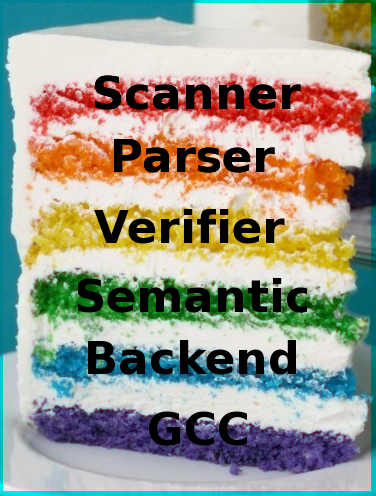
\includegraphics[width=40mm]{figures/layers.png}
\caption{A diagram showing the layers of \sys{}. The raw source code is
fed into the top of the cake and binary executables come out the bottom.
This image was manipulated by \sys{} using a Gaussian blur filter.}
\label{fig:layers}
\end{center}
\end{wrapfigure}

Our design incorporates six layers: the scanner, the parser, the verifier,
the semantic converter, the backend C generation, and C image manipulation
libraries (see Figure~\ref{fig:layers}). The compiler takes as input
a text file containing a valid \sys{} program and outputs a binary that
implements the program described by the input text.

The scanner generates as its output a one-dimensional list of
tokens (see Figure~\ref{fig:tokens}).

\begin{figure}
\begin{center}
\begin{tabular}{l l l l l l l}

    SEMI & LPAREN & RPAREN & LTCHAR & GTCHAR & LBRKT & RBRKT \\
    LBRACE & RBRACE COLON & COMMA & FSLASH & CONVOP & PIPE \\
    ATSYM & UMINUS & UPLUS & ASSIGN & DEFINE & OREQUAL & IMAGET \\
    KERNELT & CALCT & CHANNELT & UINT8T & UINT16T & UINT32T & INT8T \\
    INT16T & INT32T & ANGLET & IMGREAD & IMGWRITE & LITSTR & CSTR \\
    INTEGER & ID & EOF \\

\end{tabular}
\caption{A comprehensive list of tokens produced by the lexical analysis
(scanner).}
\end{center}
\label{fig:tokens}
\end{figure}

The parser reads this token list and uses our context-free grammar to generate
an abstract syntax tree. The parser is not strict about which nodes have
which children, or whether or not it is meaningful to have the current
structure: rather it just blindly assembles the tree. The abstract syntax tree
has the nodes described in Figure~\ref{fig:astnodes}.

\begin{figure}
\begin{center}
\begin{tabular}{l | l}
{\bf Node} & {\bf Description} \\
\hline \\
stmt & Statement \\
vdecl & Variable Declaration \\
expr & Expression \\
matrix & Calc matrix \\
bareint & Integer \\
kerncalc & Kernel calculation \\
chanref & Image channel reference \\
libfunc & \sys{} library function \\
assign\_op & Assignment operation \\
atom & Atomic type
\end{tabular}
\caption{A list of abstract syntax tree nodes.}
\label{fig:astnodes}
\end{center}
\end{figure}

The verifier accepts as input an abstract syntax tree. It traverses the
tree and checks that nodes are arranged in meaningful ways. While it
traverses, it also builds up an environment that keeps track of all
variables defined, along with their identifier name and type. If the
verifier accepts the AST, it will return as output the cumulative
environment that contains the identifiers and their types.

The semantic converter takes in a verified abstract syntax tree and also the
list of variables generated by the verifier. It then maps each node or
configuration of nodes to a corresponding Semantic AST node that
corresponds more directly with the eventual C code that must be generated.
The output of this layer is a semantically checked abstract syntax tree
(SAST). The semantic converter also supplements the environment information
inherited from the verifier with additional information not related to
verification, such the largest referenced command-line argument.

% TODO: Mapping of AST -> SAST ??

The backend takes as input the SAST and the supplemented environment
information. It then converts this into a meaningful C++ program source
file. This program can be submitted to GCC and compiled.

The final layer of \sys{} is the GCC compiler. The generated C source from
the backend is fed into the GCC compiler, which outputs a binary in
architecture-specific assembly language.

The lead developers for each layer of \sys{} are identified in
Figure~\ref{fig:leads}.


\begin{figure}
\begin{center}
\begin{tabular}{l | l}
{\bf Layer} & {\bf Lead Developer} \\
\hline \\
Unit Tests & Kevin and Yongxu \\
Scanner & Jeremy \\
Parser & Jeremy \\
Verifier & Jeremy \\
Semantic & Robert \\
Backend & Robert \\
GCC & Richard Stallman et al. \\
\end{tabular}
\caption{Who Did What: The lead developer of each layer.}
\end{center}
\label{fig:leads}
\end{figure}



    \chapter{Test Plan}
\label{chap:testplan}

Our unit test framework consists of pairs of identically named files in the \texttt{clam/tests/} directory.
Each pair consists of a CLAM program with extension \texttt{.clam} and an executable shell script
with extension \texttt{.test}. The CLAM file contains the code to be tested, while the shell script
specifies how to test that code: whether to compile and run or only compile, whether the test is supposed to fail,
what the expected output should look like, and what command line arguments to pass.
The \texttt{_buildup.sh} sets up the testing environment and defines common procedures such as
\texttt{compile-it} and \texttt{run-it}. Furthermore, \texttt{all.test} runs all tests in the directory,
tallies successes and failures and outputs a summary at the end.

Our testing is divided into four sections: syntax verification (section~\ref{testing:syntax}),
semantic/type verification (section~\ref{testing:semantic}),
CString verification (section~\ref{testing:cstrings}),
and functional output verification (section~\ref{testing:output}) which tests image processing results by comparison.

\section{Syntax Verification}
\label{testing:syntax}

Syntax verification testing is meant to confirm that the parser accepts all valid token strings,
and rejects all invalid ones as defined in our language reference manual.
We achieve this by inspecting \texttt{clam/parser.mly} and writing unit tests for
potentially problematic cases (many of the more straightforward rules were not deemed test-worthy).
All of these tests are only compiled and not executed. The testing process uncovered a number of errors
in matrix parsing and definition of kernel calculation lists.\\

\begin{itemize}

\item \texttt{matrix1.clam} tests that a simple matrix parses correctly, and should compile:
\lstinputlisting[language=CLAM]{../clam/tests/matrix1.clam}
(This originally failed because a scale factor was required, but now it is accepted.)

\item \texttt{matrix2.clam} tests that a matrix with scaling factor parses correctly, and should compile:
\lstinputlisting[language=CLAM]{../clam/tests/matrix2.clam}

\item \texttt{matrix3.clam} tests whether the parser catches ill-formed matrices, and should not compile:
\lstinputlisting[language=CLAM]{../clam/tests/matrix3.clam}
(This originally succeeded due to incorrect matrix parsing rules, but now it fails.)

\item \texttt{matrix4.clam} tests whether the parser catches another type of ill-formed matrix, and should also not compile:
\lstinputlisting[language=CLAM]{../clam/tests/matrix4.clam}
(This originally succeeded due to incorrect matrix parsing rules, but now it fails.)

\item \texttt{keyword-id.clam} tests whether the parser allows keywords to be identifiers, and should not compile:
\lstinputlisting[language=CLAM]{../clam/tests/keyword-id.clam}

\item \texttt{1calc-ker.clam} tests whether the parser allows \texttt{Kernel} definitions with only one \texttt{Calc}, and should compile:
\lstinputlisting[language=CLAM]{../clam/tests/keyword-id.clam}
(This originally failed because the original syntax caused reduce/reduce errors, so we changed both the parser and the test.
There was originally no \texttt{|} after the \texttt{=}.)

\item\texttt{string1.clam} checks that consecutive string literals are
  concatenated together into a single string literal. This should compile:
\lstinputlisting[language=CLAM]{../clam/tests/string1.clam}

\item \texttt{convoperand.clam} tests whether the \texttt{**} enforces a strict order of operands, and should not compile:
\lstinputlisting[language=CLAM]{../clam/tests/convoperand.clam}
(We only allow convolutions of the form \emph{channel-ref} \texttt{**} \emph{identifier}, in order to simplify
to translation into C code.)

\item \texttt{defcalc1.clam}, \texttt{defcalc2.clam}, and \texttt{defcalc3.clam} test various ways of declaring \texttt{Calc}s,
and all three should compile:
\lstinputlisting[language=CLAM]{../clam/tests/defcalc1.clam}
\lstinputlisting[language=CLAM]{../clam/tests/defcalc2.clam}
\lstinputlisting[language=CLAM]{../clam/tests/defcalc3.clam}

\item \texttt{rval-calc.clam}, \texttt{rval-matrix.clam}, \texttt{rval-chanref.clam}, \texttt{rval-conv.clam},
\texttt{rval-cstr.clam}, \texttt{rval-image.clam}, \texttt{rval-imgread.clam}, and \texttt{rval-kernel.clam}
test various "do nothing" statements consisting solely of r-values. Theses should all compile, though their
return values of the last line of each test are discarded so they do nothing:
\lstinputlisting[language=CLAM]{../clam/tests/rval-calc.clam}
\lstinputlisting[language=CLAM]{../clam/tests/rval-matrix.clam}
\lstinputlisting[language=CLAM]{../clam/tests/rval-chanref.clam}
\lstinputlisting[language=CLAM]{../clam/tests/rval-conv.clam}
\lstinputlisting[language=CLAM]{../clam/tests/rval-cstr.clam}
\lstinputlisting[language=CLAM]{../clam/tests/rval-image.clam}
\lstinputlisting[language=CLAM]{../clam/tests/rval-imgread.clam}
\lstinputlisting[language=CLAM]{../clam/tests/rval-kernel.clam}
(The parser accepted all of these, though most originally caused errors in the C translator
that had to be fixed (see "C Compiler Verification" below).)

\item \texttt{equality-trans.clam} checks that assignment expressions can be nested. This should compile:
\lstinputlisting[language=CLAM]{../clam/tests/equality-trans.clam}

\item \texttt{comment1.clam} checks that a program with only a comment (and zero statements) compiles. This should compile:
\lstinputlisting[language=CLAM]{../clam/tests/comment1.clam}

\end{itemize}

\section{Semantic Verification}
\label{testing:semantic}

Semantic verification testing is meant to confirm that the verifier accepts all valid parse trees,
and rejects all invalid ones according to the specifications of our language
(and according to what makes sense).
These tests depend on \texttt{clam/verifier.ml}, as well as \texttt{clam/environ.ml} and \texttt{envtypes.mli}. 
The testing process uncovered a number of errors in matrix verification (separate from syntax)
and the creation of default RGB Channels.\\

\begin{itemize}

\item\texttt{zerocalc1.clam} and \texttt{zerocalc2.clam} check that a matrix scaling-factor can
have a numerator of zero, but not a denominator of zero.
The former should certainly compile, while the latter should not:
\lstinputlisting[language=CLAM]{../clam/tests/zerocalc1.clam}
\lstinputlisting[language=CLAM]{../clam/tests/zerocalc2.clam}
(\texttt{zerocalc2.clam} originally passed verification, but that was fixed.)

\item\texttt{invalid1.clam} checks that undeclared identifiers are caught. This should not compile:
\lstinputlisting[language=CLAM]{../clam/tests/invalid1.clam}

\item\texttt{undefined1.clam} checks that an undefined Channel reference cannot be an r-value. This should not compile:
\lstinputlisting[language=CLAM]{../clam/tests/undefined1.clam}

\item\texttt{imgchannel1.clam} checks that an \texttt{Image} has default channels when read. This should compile:
\lstinputlisting[language=CLAM]{../clam/tests/imgchannel1.clam}

\item\texttt{imgchannel2.clam} checks that an undefined \texttt{Calc} cannot be applied to an \texttt{Image}. This should not compile:
\lstinputlisting[language=CLAM]{../clam/tests/imgchannel2.clam}

\item\texttt{imgchannel3.clam} checks that a \texttt{Calc} defined as a matrix cannot be applied to an \texttt{Image}. This should not compile:
\lstinputlisting[language=CLAM]{../clam/tests/imgchannel3.clam}

\item\texttt{imgchannel4.clam} checks that a \texttt{Calc} defined as a CString \emph{can} be applied to an \texttt{Image}. This should compile:
\lstinputlisting[language=CLAM]{../clam/tests/imgchannel4.clam}

\item\texttt{image-eq-image.clam} checks \texttt{=} assignment for images to images. This should compile:
\lstinputlisting[language=CLAM]{../clam/tests/image-eq-image.clam}

\item\texttt{image-oreq-image.clam} checks \texttt{|=} assignment for images to images. This is not supported and doesn't compile:
\lstinputlisting[language=CLAM]{../clam/tests/image-oreq-image.clam}

\item\texttt{image-defeq.clam} checks \texttt{:=} assignment for images. This is not supported and doesn't compile:
\lstinputlisting[language=CLAM]{../clam/tests/image-defeq.clam}

\item\texttt{imgread-bad.clam} checks that l-value identifiers have to be declared first. This shouldn't compile:
\lstinputlisting[language=CLAM]{../clam/tests/imgread-bad.clam}

\item\texttt{imgread-bad2.clam} checks that \texttt{imgread} must be called with only one argument. This shouldn't compile:
\lstinputlisting[language=CLAM]{../clam/tests/imgread-bad2.clam}

\item\texttt{imgread-bad3.clam} checks that \texttt{imgread} can only be called with a literal string or integer. This shouldn't compile:
\lstinputlisting[language=CLAM]{../clam/tests/imgread-bad3.clam}

\item\texttt{imgread.clam} checks that \texttt{imgread} can actually called with a correct argument. This should compile:
\lstinputlisting[language=CLAM]{../clam/tests/imgread-bad.clam}

\item\texttt{imgwrite-bad1.clam} checks that \texttt{imgwrite} can't be called with incorrect number and type of arguments. This shouldn't compile:
\lstinputlisting[language=CLAM]{../clam/tests/imgwrite-bad1.clam}

\item\texttt{defchannels.clam} checks that the default RGB Channels don't exist for a declared-but-not-read \texttt{Image}. This shouldn't compile:
\lstinputlisting[language=CLAM]{../clam/tests/defchannels.clam}
(Allowing default RGB channels for an unread \texttt{Image} is problematic because CLAM
does not allow explicit manipulation of Channel \emph{size}.)

\item\texttt{imgwrite-norgb.clam} checks that a declared-but-not-read \texttt{Image} without RGB channels
(and more importantly, without a \emph{size}) cannot be written. This shouldn't compile:
\lstinputlisting[language=CLAM]{../clam/tests/imgwrite-norgb.clam}

\item\texttt{sizediff.clam} checks that the default Channels from \texttt{Image}s of different sizes
cannot be assigned to each other, because all Channels of an \texttt{Image} should have the same size. This shouldn't compile:
\lstinputlisting[language=CLAM]{../clam/tests/sizediff.clam}

\item\texttt{at-channel.clam} checks that transient \texttt{Calc}s marked with \texttt{@} in a \texttt{Kernel}
do not result in Channels after a convolution. This shouldn't compile:
\lstinputlisting[language=CLAM]{../clam/tests/at-channel.clam}

\item\texttt{addker.clam} checks a \texttt{Kernel} can be appended to another \texttt{Kernel} using \texttt{|=}. This should compile:
\lstinputlisting[language=CLAM]{../clam/tests/addker.clam}

\item\texttt{DefEq.clam} checks that \texttt{=} cannot be used to define a \texttt{Calc}. This should not compile:
\lstinputlisting[language=CLAM]{../clam/tests/DefEq.clam}

\item\texttt{ckernel.clam} checks that \texttt{Kernel}s must be defined using \texttt{Calc} \emph{identifiers}
and not anonymous \texttt{Calc} expressions. This should not compile:
\lstinputlisting[language=CLAM]{../clam/tests/ckernel.clam}

\item\texttt{cimage.clam} checks that \texttt{Image}s cannot be defined using \texttt{Calc} expressions. This should not compile:
\lstinputlisting[language=CLAM]{../clam/tests/cimage.clam}

\end{itemize}

\section{CString Verification}
\label{testing:cstrings}

CString verification testing checks that invalid CStrings are caught before being passed to GCC, where they
could cause fatal errors. Of course, it is impossible to catch \emph{all} possible errors without
building an understanding of C syntax directly into CLAM, so we are satisfied with catching common
mistakes and rely on the user and GCC error messages for everything else. (For example, a CString of the form \texttt{\#[while(1)]\#},
while certainly disruptive, will compile and it is the user's fault that the program stalls.)
For each possible issue that we \emph{did} choose to catch, we wrote unit tests to confirm that they were caught.
Catching of invalid CStrings is done entirely in \texttt{clam/scanner.mll}. Testing reveals errors
in parentheses matching, which were promptly corrected.\\

\begin{itemize}

\item\texttt{cstring1.clam} checks that C preprocessor cannot be used in a CString. This should not compile:
\lstinputlisting[language=CLAM]{../clam/tests/cstring1.clam}

\item\texttt{cstring2.clam} checks that C comments cannot be used in a CString. This should not compile:
\lstinputlisting[language=CLAM]{../clam/tests/cstring2.clam}

\item\texttt{cstring3.clam} checks that empty CStrings are OK, and just result in an empty statement. This should compile:
\lstinputlisting[language=CLAM]{../clam/tests/cstring3.clam}

\item\texttt{cstring4.clam} checks that library calls in a CString must be closed. This should not compile:
\lstinputlisting[language=CLAM]{../clam/tests/cstring4.clam}
(This originally did compile because the scanner didn't record nesting-level properly. It was fixed.)

\item\texttt{cstring5.clam} checks that parentheses in a CString must be matched. This should not compile:
\lstinputlisting[language=CLAM]{../clam/tests/cstring5.clam}
(This originally did compile because the scanner didn't record nesting-level properly. It was fixed.)

\item\texttt{cstring6.clam} is a sanity check that "normal" CStrings do in fact work. This should obviously compile:
\lstinputlisting[language=CLAM]{../clam/tests/cstring6.clam}

\end{itemize}

\section{C Compiler Verification}
\label{testing:ccompiler}

A few of the above tests, which originally compiled, began failing once the C backend was hooked up.
The most common errors were with C syntax and memory allocation.
While we didn't write tests specifically targeted at the C backend,
the tests we wrote for other parts of the architecture also helped us identify problems in the C translator. 

\section{Image Processing Verification}
\label{testing:output}

These are comprehensive tests, consisting of full-fledged programs that actually
read, manipulate and write images. While the testing framework provides image-comparison functionality,
most verification here is actually done with the naked eye.\\

\begin{itemize}

\item\texttt{imgcopy.clam} copies an image. This should compile, run, and copy an image:
\lstinputlisting[language=CLAM]{../clam/tests/imgcopy.clam}

\item\texttt{sobel.clam} applies the Sobel operation to an image. This should compile, run, and output
a map of the luminosity gradient:
\lstinputlisting[language=CLAM]{../clam/tests/sobel.clam}

\end{itemize}



    \chapter{Lessons Learned}


    \appendix
    \chapter{Complete Code Reference}
\label{chap:coderef}
The \sys{} programming language was implemented in OCaml. It uses the
C/C++ programming languages as backend targets, and invokes the \texttt{g++}
compiler on the \sys{} compilation output to produce a final binary. The
final binary is statically linked against a \sys{} implementation library,
\texttt{clam.a}, which contains the low-level image manipulation functions. Additionally,
\sys{} leveraged several OCaml functions from the \emph{extlib}~\cite{extlib:googlecode}
project, and a stand-alone image reader~\cite{stbimage:read} and writer~\cite{stbimage:write}
library written by Sean Barrett. Code listings of the \sys{} compiler and \sys{} implementation library
as well as the subset of \emph{extlib} used by \sys{} follow:

\clearpage
\section{\sys{} Compiler}
\lstinputlisting[language=Ocaml]{../clam/clam.ml} \clearpage
\lstinputlisting[language=Ocaml]{../clam/ast.mli} \clearpage
\lstinputlisting[language=Ocaml]{../clam/backend.ml} \clearpage
\lstinputlisting[language=Ocaml]{../clam/clamsys.ml} \clearpage
\lstinputlisting[language=Ocaml]{../clam/environ.ml} \clearpage
\lstinputlisting[language=Ocaml]{../clam/envtypes.mli} \clearpage
\lstinputlisting[language=Ocaml]{../clam/parseutil.ml} \clearpage
\lstinputlisting[language=Ocaml]{../clam/parser.mly} \clearpage
\lstinputlisting[language=Ocaml]{../clam/printer.ml} \clearpage
\lstinputlisting[language=Ocaml]{../clam/sast.mli} \clearpage
\lstinputlisting[language=Ocaml]{../clam/scanner.mll} \clearpage
\lstinputlisting[language=Ocaml]{../clam/semantic.ml} \clearpage
\lstinputlisting[language=Ocaml]{../clam/verifier.ml} \clearpage

\subsection{Subset of \emph{extlib} Used by \sys{}}
\sys{} compiled the following source files from the \texttt{extlib}~\cite{extlib:googlecode}
project. Their full source is omitted for brevity -- see the project website.
\begin{itemize}
  \item{\texttt{enum.ml}}
  \item{\texttt{enum.mli}}
  \item{\texttt{extString.ml}}
  \item{\texttt{extString.mli}}
  \item{\texttt{std.ml}}
  \item{\texttt{std.mli}}
\end{itemize}
\comment{
  \lstinputlisting[language=Ocaml]{../clam/extlib/enum.ml} \clearpage
  \lstinputlisting[language=Ocaml]{../clam/extlib/enum.mli} \clearpage
  \lstinputlisting[language=Ocaml]{../clam/extlib/extString.ml} \clearpage
  \lstinputlisting[language=Ocaml]{../clam/extlib/extString.mli} \clearpage
  \lstinputlisting[language=Ocaml]{../clam/extlib/std.ml} \clearpage
  \lstinputlisting[language=Ocaml]{../clam/extlib/std.mli} \clearpage
} % END-COMMENT

\section{\sys{} Implementation Library (\texttt{clam.a})}
\definecolor{cstyleDarkRed}{rgb}{0.65, 0.08, 0.0}
\definecolor{cstyleDarkBlue}{rgb}{0.0, 0.08, 0.65}
\definecolor{cstyleGrey}{rgb}{0.55, 0.55, 0.55}
\lstset{
    keywordstyle={\color{cstyleDarkRed}\bfseries},
    commentstyle={\color{cstyleGrey}\bfseries},
    %directivestyle={\color{cstyleDarkBlue}},
    sensitive=true,
    showstringspaces=false,
    showspaces=false,
    showtabs=false,
    numbers=left,
    frame=single,
    breaklines=true,
    basicstyle=\ttfamily\scriptsize,
}
%\subsection{\sys{} C Source}
\lstinputlisting[language=C]{../clam/libstb/clam.h} \clearpage
\lstinputlisting[language=C]{../clam/libstb/clam.c} \clearpage
%\subsection{\texttt{stb\_image} Source}
%\lstinputlisting[language=C]{../clam/libstb/stb-image-read.c} \clearpage
%\lstinputlisting[language=C]{../clam/libstb/stb-image-write.c} \clearpage

\section{Unit Test Framework}
Our unit testing framework was built on two custom shell scripts that provided
a framework to compile a test program, determine success/failure of compilation,
compare image outputs and report overall success or failure of the test.
The framework simply runs all shell scripts in the \emph{test} directory and
reports the success/failure of each one (with a summary of failures at the end).
The \texttt{_buildup.sh}, \texttt{_breakdown.sh}, and \texttt{all.test} scripts are
reported here, followed by all of the tests and a sample run of the
\texttt{all.test} script.
\vskip -4mm

\vskip -4mm
\subsection*{_buildup.sh}
\vskip -2mm
\lstinputlisting[language=bash]{../clam/tests/build-up-script-link.sh} \clearpage
\subsection*{_breakdown.sh}
\lstinputlisting[language=bash]{../clam/tests/breakdown-script-link.sh}
\subsection*{all.test}
\lstinputlisting[language=bash]{../clam/tests/all.test} \clearpage
% all the tests 
\subsection*{The tests (shell script followed by \sys{} source)}
\subsection*{Unit Test: 1calc-ker}
\lstinputlisting[language=bash]{../clam/tests/1calc-ker.test}
\lstinputlisting[language=bash]{../clam/tests/1calc-ker.clam} \clearpage
\subsection*{Unit Test: DefEq}
\lstinputlisting[language=bash]{../clam/tests/DefEq.test}
\lstinputlisting[language=bash]{../clam/tests/DefEq.clam} \clearpage
\subsection*{Unit Test: addker}
\lstinputlisting[language=bash]{../clam/tests/addker.test}
\lstinputlisting[language=bash]{../clam/tests/addker.clam} \clearpage
\subsection*{Unit Test: at-channel}
\lstinputlisting[language=bash]{../clam/tests/at-channel.test}
\lstinputlisting[language=bash]{../clam/tests/at-channel.clam} \clearpage
\subsection*{Unit Test: cimage}
\lstinputlisting[language=bash]{../clam/tests/cimage.test}
\lstinputlisting[language=bash]{../clam/tests/cimage.clam} \clearpage
\subsection*{Unit Test: ckernel}
\lstinputlisting[language=bash]{../clam/tests/ckernel.test}
\lstinputlisting[language=bash]{../clam/tests/ckernel.clam} \clearpage
\subsection*{Unit Test: comment1}
\lstinputlisting[language=bash]{../clam/tests/comment1.test}
\lstinputlisting[language=bash]{../clam/tests/comment1.clam} \clearpage
\subsection*{Unit Test: convoperand}
\lstinputlisting[language=bash]{../clam/tests/convoperand.test}
\lstinputlisting[language=bash]{../clam/tests/convoperand.clam} \clearpage
\subsection*{Unit Test: cstring1}
\lstinputlisting[language=bash]{../clam/tests/cstring1.test}
\lstinputlisting[language=bash]{../clam/tests/cstring1.clam} \clearpage
\subsection*{Unit Test: cstring2}
\lstinputlisting[language=bash]{../clam/tests/cstring2.test}
\lstinputlisting[language=bash]{../clam/tests/cstring2.clam} \clearpage
\subsection*{Unit Test: cstring3}
\lstinputlisting[language=bash]{../clam/tests/cstring3.test}
\lstinputlisting[language=bash]{../clam/tests/cstring3.clam} \clearpage
\subsection*{Unit Test: cstring4}
\lstinputlisting[language=bash]{../clam/tests/cstring4.test}
\lstinputlisting[language=bash]{../clam/tests/cstring4.clam} \clearpage
\subsection*{Unit Test: cstring5}
\lstinputlisting[language=bash]{../clam/tests/cstring5.test}
\lstinputlisting[language=bash]{../clam/tests/cstring5.clam} \clearpage
\subsection*{Unit Test: cstring6}
\lstinputlisting[language=bash]{../clam/tests/cstring6.test}
\lstinputlisting[language=bash]{../clam/tests/cstring6.clam} \clearpage
\subsection*{Unit Test: defcalc1}
\lstinputlisting[language=bash]{../clam/tests/defcalc1.test}
\lstinputlisting[language=bash]{../clam/tests/defcalc1.clam} \clearpage
\subsection*{Unit Test: defcalc2}
\lstinputlisting[language=bash]{../clam/tests/defcalc2.test}
\lstinputlisting[language=bash]{../clam/tests/defcalc2.clam} \clearpage
\subsection*{Unit Test: defcalc3}
\lstinputlisting[language=bash]{../clam/tests/defcalc3.test}
\lstinputlisting[language=bash]{../clam/tests/defcalc3.clam} \clearpage
\subsection*{Unit Test: defchannels}
\lstinputlisting[language=bash]{../clam/tests/defchannels.test}
\lstinputlisting[language=bash]{../clam/tests/defchannels.clam} \clearpage
\subsection*{Unit Test: equality-trans}
\lstinputlisting[language=bash]{../clam/tests/equality-trans.test}
\lstinputlisting[language=bash]{../clam/tests/equality-trans.clam} \clearpage
\subsection*{Unit Test: id-overlap}
\lstinputlisting[language=bash]{../clam/tests/id-overlap.test}
\lstinputlisting[language=bash]{../clam/tests/id-overlap.clam} \clearpage
\subsection*{Unit Test: image-defeq}
\lstinputlisting[language=bash]{../clam/tests/image-defeq.test}
\lstinputlisting[language=bash]{../clam/tests/image-defeq.clam} \clearpage
\subsection*{Unit Test: image-eq-image}
\lstinputlisting[language=bash]{../clam/tests/image-eq-image.test}
\lstinputlisting[language=bash]{../clam/tests/image-eq-image.clam} \clearpage
\subsection*{Unit Test: image-oreq-image}
\lstinputlisting[language=bash]{../clam/tests/image-oreq-image.test}
\lstinputlisting[language=bash]{../clam/tests/image-oreq-image.clam} \clearpage
\subsection*{Unit Test: imgchannel1}
\lstinputlisting[language=bash]{../clam/tests/imgchannel1.test}
\lstinputlisting[language=bash]{../clam/tests/imgchannel1.clam} \clearpage
\subsection*{Unit Test: imgchannel2}
\lstinputlisting[language=bash]{../clam/tests/imgchannel2.test}
\lstinputlisting[language=bash]{../clam/tests/imgchannel2.clam} \clearpage
\subsection*{Unit Test: imgchannel3}
\lstinputlisting[language=bash]{../clam/tests/imgchannel3.test}
\lstinputlisting[language=bash]{../clam/tests/imgchannel3.clam} \clearpage
\subsection*{Unit Test: imgchannel4}
\lstinputlisting[language=bash]{../clam/tests/imgchannel4.test}
\lstinputlisting[language=bash]{../clam/tests/imgchannel4.clam} \clearpage
\subsection*{Unit Test: imgcopy}
\lstinputlisting[language=bash]{../clam/tests/imgcopy.test}
\lstinputlisting[language=bash]{../clam/tests/imgcopy.clam} \clearpage
\subsection*{Unit Test: imgread}
\lstinputlisting[language=bash]{../clam/tests/imgread.test}
\lstinputlisting[language=bash]{../clam/tests/imgread.clam} \clearpage
\subsection*{Unit Test: imgread-bad}
\lstinputlisting[language=bash]{../clam/tests/imgread-bad.test}
\lstinputlisting[language=bash]{../clam/tests/imgread-bad.clam} \clearpage
\subsection*{Unit Test: imgread-bad2}
\lstinputlisting[language=bash]{../clam/tests/imgread-bad2.test}
\lstinputlisting[language=bash]{../clam/tests/imgread-bad2.clam} \clearpage
\subsection*{Unit Test: imgread-bad3}
\lstinputlisting[language=bash]{../clam/tests/imgread-bad3.test}
\lstinputlisting[language=bash]{../clam/tests/imgread-bad3.clam} \clearpage
\subsection*{Unit Test: imgwrite-bad1}
\lstinputlisting[language=bash]{../clam/tests/imgwrite-bad1.test}
\lstinputlisting[language=bash]{../clam/tests/imgwrite-bad1.clam} \clearpage
\subsection*{Unit Test: imgwrite-norgb}
\lstinputlisting[language=bash]{../clam/tests/imgwrite-norgb.test}
\lstinputlisting[language=bash]{../clam/tests/imgwrite-norgb.clam} \clearpage
\subsection*{Unit Test: invalid1}
\lstinputlisting[language=bash]{../clam/tests/invalid1.test}
\lstinputlisting[language=bash]{../clam/tests/invalid1.clam} \clearpage
\subsection*{Unit Test: keyword-id}
\lstinputlisting[language=bash]{../clam/tests/keyword-id.test}
\lstinputlisting[language=bash]{../clam/tests/keyword-id.clam} \clearpage
\subsection*{Unit Test: matrix1}
\lstinputlisting[language=bash]{../clam/tests/matrix1.test}
\lstinputlisting[language=bash]{../clam/tests/matrix1.clam} \clearpage
\subsection*{Unit Test: matrix2}
\lstinputlisting[language=bash]{../clam/tests/matrix2.test}
\lstinputlisting[language=bash]{../clam/tests/matrix2.clam} \clearpage
\subsection*{Unit Test: matrix3}
\lstinputlisting[language=bash]{../clam/tests/matrix3.test}
\lstinputlisting[language=bash]{../clam/tests/matrix3.clam} \clearpage
\subsection*{Unit Test: matrix4}
\lstinputlisting[language=bash]{../clam/tests/matrix4.test}
\lstinputlisting[language=bash]{../clam/tests/matrix4.clam} \clearpage
\subsection*{Unit Test: rval-calc}
\lstinputlisting[language=bash]{../clam/tests/rval-calc.test}
\lstinputlisting[language=bash]{../clam/tests/rval-calc.clam} \clearpage
\subsection*{Unit Test: rval-chanref}
\lstinputlisting[language=bash]{../clam/tests/rval-chanref.test}
\lstinputlisting[language=bash]{../clam/tests/rval-chanref.clam} \clearpage
\subsection*{Unit Test: rval-conv}
\lstinputlisting[language=bash]{../clam/tests/rval-conv.test}
\lstinputlisting[language=bash]{../clam/tests/rval-conv.clam} \clearpage
\subsection*{Unit Test: rval-cstr}
\lstinputlisting[language=bash]{../clam/tests/rval-cstr.test}
\lstinputlisting[language=bash]{../clam/tests/rval-cstr.clam} \clearpage
\subsection*{Unit Test: rval-image}
\lstinputlisting[language=bash]{../clam/tests/rval-image.test}
\lstinputlisting[language=bash]{../clam/tests/rval-image.clam} \clearpage
\subsection*{Unit Test: rval-imgread}
\lstinputlisting[language=bash]{../clam/tests/rval-imgread.test}
\lstinputlisting[language=bash]{../clam/tests/rval-imgread.clam} \clearpage
\subsection*{Unit Test: rval-kernel}
\lstinputlisting[language=bash]{../clam/tests/rval-kernel.test}
\lstinputlisting[language=bash]{../clam/tests/rval-kernel.clam} \clearpage
\subsection*{Unit Test: rval-matrix}
\lstinputlisting[language=bash]{../clam/tests/rval-matrix.test}
\lstinputlisting[language=bash]{../clam/tests/rval-matrix.clam} \clearpage
\subsection*{Unit Test: sizediff}
\lstinputlisting[language=bash]{../clam/tests/sizediff.test}
\lstinputlisting[language=bash]{../clam/tests/sizediff.clam} \clearpage
\subsection*{Unit Test: sobel}
\lstinputlisting[language=bash]{../clam/tests/sobel.test}
\lstinputlisting[language=bash]{../clam/tests/sobel.clam} \clearpage
\subsection*{Unit Test: undefined1}
\lstinputlisting[language=bash]{../clam/tests/undefined1.test}
\lstinputlisting[language=bash]{../clam/tests/undefined1.clam} \clearpage
\subsection*{Unit Test: zerocalc1}
\lstinputlisting[language=bash]{../clam/tests/zerocalc1.test}
\lstinputlisting[language=bash]{../clam/tests/zerocalc1.clam} \clearpage
\subsection*{Unit Test: zerocalc2}
\lstinputlisting[language=bash]{../clam/tests/zerocalc2.test}
\lstinputlisting[language=bash]{../clam/tests/zerocalc2.clam} \clearpage

\chapter{Project Version Control History}
\label{chap:vcshistory}
The \sys{} project used \texttt{git}~\cite{git:website} as its version control system.
Here we provide the output of the \texttt{git-shortlog} program with \emph{Merge}
commits filtered out, followed by a more complete revision control history.

%
% clam.tex -- master LaTeX file for 'CLAM: The Concise Linear Algebra Manipulation Language'
%
\newcommand{\sys}{CLAM}
\newcommand{\longtitle}{\sys{}: The Concise Linear Algebra Manipulation Language}
\newcommand{\authorlist}{Jeremy Andrus and Robert Martin and Kevin Sun and Yongxu Zhang}
\newcommand{\authoremails}{\{jca2119, rdm2128, kfs2110, yz2419\}@columbia.edu}

% Build Project proposal only (default for now)
\ifcsname ifproposal\endcsname\else
  \expandafter\let\csname ifproposal\expandafter\endcsname
                  \csname iftrue\endcsname
\fi
% Build Language Reference Manual only
\ifcsname ifrefman\endcsname\else
  \expandafter\let\csname ifrefman\expandafter\endcsname
                  \csname iffalse\endcsname
\fi
\ifcsname ifbook\endcsname\else
  \expandafter\let\csname ifbook\expandafter\endcsname
                  \csname iffalse\endcsname
\fi

% Document Class
\ifbook
  \documentclass[10pt,letterpaper,titlepage,onecolumn,oneside]{book}
\else
  \documentclass[10pt,letterpaper,onecolumn,oneside]{article}
\fi

\usepackage[margin=1.0in]{geometry}
\usepackage[utf8x]{inputenc}
\usepackage{ucs}
\usepackage{amsmath}
\usepackage{amsfonts}
\usepackage{amssymb}
\usepackage[usenames,dvipsnames]{color}
\usepackage{listings}
\usepackage[font=scriptsize,caption=false]{subfig}
\usepackage{underscore}
% hyphenat redefines "BreakableUnderscore", so I need
% to do some LaTeX gymnastics to make it work...
\makeatletter
\let\BreakableUnderscore\@undefined
\makeatother
\usepackage{hyphenat}
\usepackage{wrapfig}
\usepackage{lastpage}
\usepackage{balance}
\usepackage{cite}
\usepackage{pdfsync}
\usepackage[colorlinks=false,
    pdftitle={\longtitle{}},
    pdfborder={0 0 0},
    pdfauthor={\authorlist{}},
    pdfdisplaydoctitle=true,
    plainpages=false]{hyperref}
\usepackage{breakurl}
\usepackage{multirow}
\usepackage{pgfgantt}

\setlength{\parindent}{0in}
\addtolength{\parskip}{\baselineskip}

% other useful commands
\newcommand{\comment}[1]{}

\begin{document}

% this usually saves about a line-or-two by squeezing inter-sentence space
%\frenchspacing

\title{\longtitle{}}
\author{\authorlist{}\\\authoremails{}\\\\Columbia University\\COMS W4115: Programming Languages and Translators}
\maketitle

% Body of the paper in different files
\ifproposal
  % Project Proposal
  \section*{Language Proposal}

\definecolor{DarkBlue}{rgb}{0.0, 0.08, 0.65}
\definecolor{DarkRed}{rgb}{0.65, 0.08, 0.0}
\definecolor{DarkGreen}{rgb}{0.08, 0.35, 0.08}
\definecolor{Grey}{rgb}{0.55, 0.55, 0.55}
\definecolor{Yellow}{cmyk}{0.0, 0.08, 0.5, 0.3}
\definecolor{Brown}{rgb}{0.55, 0.27, 0.08}
\definecolor{LightBlue}{cmyk}{0.8, 0.1, 0.0, 0.1}
\lstdefinelanguage{PLTF11}{
    classoffset=0,
	morekeywords={somethingsomethingsomething},
    keywordstyle={\color{Yellow}\itshape\bfseries},
    classoffset=1,
    morekeywords={Uint8,Uint16,Uint32,Int8,Int16,Int32,Angle,Matrix,Image,Kernel},
    keywordstyle={\color{DarkBlue}\bfseries},
    classoffset=2,
	morekeywords={imgread,imgwrite},
	keywordstyle={\color{Brown}},
	otherkeywords={:=,**,=,|,:},
	moredelim=*[s][\color{LightBlue}]{\#[}{]},
	moredelim=*[s][\color{DarkGreen}\itshape]{\$(}{)},
    morecomment=[l]{//},
    commentstyle={\color{Grey}\bfseries},
    morestring=[b]",
    stringstyle={\color{DarkRed}},
    sensitive=true,
}

\comment{
Possible language names:
LIP - Linear Image Processing (+1)
MILA - Manipulate Images w/ Linear Algebra
CLAM - Color & Light Algebraic Manipulation/Convolutions, Linear Algebra & Matrices
GeBR - Middle part of "alGeBRa", and a rearrangement of RGB - because it manipulates colors.
}

\sys{} is a linear algebra manipulation language specifically targeted for
image processing. It provides an efficient way to express complex image
manipulation algorithms through compact matrix operations. Traditional image
processing is performed using a language such as C, or C++. Algorithms in these
languages are quite complex and error-prone due to the large number of lines of
code required to implement something as conceptually simple as, "make this image
blurry." The complexity arises from the need to perform elaborate calculations
on every pixel in an image. For example, to blur an image you first need to
calculate the luminance of the pixel (from the red, green, and blue channels),
then you need to mathematically combine this with the luminance of adjacent pixels,
and finally re-calculate red, green, and blue values for an output image.

\sys{} will simplify image processing, and more generally linear algebra, through
domain-specific data types and operators. The basic data type in \sys{} is a 
\texttt{Matrix}. Matrices can be manipulated by operators that perform functions
such as matrix multiplication, or rotation. An \texttt{Image} is another \sys{}
data type which is expressed as a collection of matrices, or channels. For example,
when reading an image into memory, \sys{} creates a \emph{Red}, \emph{Green}, and
\emph{Blue} channel automatically. Additional Image channels can either be assigned,
or calculated using an expression syntax which defines a calculation involving the
values of other, previously defined, channels. The basic image processing operator
in \sys{} is the convolution operator. This operator takes a channel and a
\texttt{Kernel}, another basic data type, and outputs an \texttt{Image}. This
operator convolves each \texttt{Matrix} within the \texttt{Kernel} with the input channel,
and collects the resulting output channels into an \texttt{Image}.

Two primary use cases of \sys{} are basic image information extraction, and
filtering. The compact syntax and powerful basic data types of \sys{} will make
information extraction, such as finding all the edges in an image, simple, compact,
and easy to read.

\subsection*{Features}
\sys{} uses implicit loops, i.e. there is no explicit looping construct in the
language. Loops are implicitly defined by per-pixel matrix or convolution
operations. Additionally, \sys{} automatically determines or calculates image and matrix
dimensions. There is no need to explicitly size these data types. This further
reduces complexity, and eliminates frequent mistakes such as going beyond array
bounds in a calculation.

\subsection*{Example Syntax}

The goal of the \sys{} syntax will be to make conceptually simple image
manipulations into simple language constructs. For instance, convolutions make
frequent use of constant matrices, so our language will provide a simple way
to specify them, such as:
\begin{lstlisting}[language=PLTF11]
    Matrix sobelGy := { +1 +2 +1 |  0  0  0 | -1 -2 -1 };
\end{lstlisting}

Another common image processing technique is performing the same calculation
on every pixel in the image. An example of this is calculating the luminance
of a pixel from the red, green, and blue channels. \sys{} makes this calculation
simple and compact by defining an additional image channel. Assuming there exists
an instance of a \texttt{Image} variable named, \emph{myimg}, a channel can be
added to the image with:
\begin{lstlisting}[language=PLTF11]
    Int32 myimg:Luminance := #[ (3*Red + 6*Green + 1*Blue) / 10 ];
\end{lstlisting}
Where the expression within \texttt{\#[ \ldots ]} is evaluated once for every
pixel in the \texttt{Image}. The \emph{Red}, \emph{Green}, and \emph{Blue} variables
correspond to previously defined channels in \emph{myimg}, and their values during
expression evaluation will be the value of the corresponding channel at the current
pixel location.

Image processing also frequently involves describing a series of operations that
should be carried out for each pixel, and then repeating it for every pixel in an
image. \sys{} makes it simple to describe this process through the \texttt{Kernel}
data type and the convolution operator. Here is an example of how one might perform
a Sobel edge detector in the \sys{} language:
\lstinputlisting[language=PLTF11,numbers=left,frame=single]{src/sobel.imp}

\else
  
\definecolor{clamLightBlue}{cmyk}{0.8, 0.1, 0.0, 0.1}
\definecolor{clamDarkBlue}{rgb}{0.0, 0.08, 0.65}
\definecolor{clamDarkRed}{rgb}{0.65, 0.08, 0.0}
\definecolor{clamDarkGreen}{rgb}{0.08, 0.35, 0.08}
\definecolor{clamYellow}{cmyk}{0.0, 0.08, 0.5, 0.3}
\definecolor{clamPurple}{rgb}{0.58, 0.0, 0.83}
\definecolor{clamBrown}{rgb}{0.55, 0.27, 0.08}
\definecolor{clamGrey}{rgb}{0.55, 0.55, 0.55}
\lstdefinelanguage{CLAM}{
    classoffset=0,
    keywordstyle={\color{clamYellow}\bfseries}, % default style (used by 'otherkeywords')
    morekeywords={somethingsomethingsomething},
    classoffset=1,
    morekeywords={Uint8,Uint16,Uint32,Int8,Int16,Int32,Calc,Angle,Image,Kernel},
    keywordstyle={\color{clamDarkRed}\bfseries},
    classoffset=2,
    morekeywords={imgread,imgwrite},
    keywordstyle={\color{clamPurple}\bfseries},
    classoffset=3,
    otherkeywords={=,|,\,,:,:=,**,@},
    morecomment=[l]{//},
    morecomment=[n]{/*}{*/},
    commentstyle={\color{clamGrey}\bfseries},
    morestring=[b]",
    stringstyle={\color{clamBrown}},
    moredelim=*[s][\color{clamLightBlue}]{\#[}{]\#},
    moredelim=*[s][\color{clamBrown}]{[}{]},
    moredelim=*[s][\color{clamDarkGreen}]{\{}{\};},
    sensitive=true,
    showstringspaces=false,
    showspaces=false,
    showtabs=false,
    frame=single,
    numbers=left,
    basicstyle=\ttfamily,
}


  % Adapted from vim Ocaml syntax highlighting

\definecolor{ocamlLightBlue}{cmyk}{0.8, 0.1, 0.0, 0.1}
\definecolor{ocamlDarkBlue}{rgb}{0.0, 0.08, 0.65}
\definecolor{ocamlDarkRed}{rgb}{0.65, 0.08, 0.0}
\definecolor{ocamlDarkGreen}{rgb}{0.08, 0.35, 0.08}
\definecolor{ocamlYellow}{cmyk}{0.0, 0.08, 0.5, 0.3}
\definecolor{ocamlPurple}{rgb}{0.58, 0.0, 0.83}
\definecolor{ocamlBrown}{rgb}{0.55, 0.27, 0.08}
\definecolor{ocamlGrey}{rgb}{0.55, 0.55, 0.55}
\lstdefinelanguage{OCaml}{
    classoffset=0,
    keywordstyle={\color{ocamlPurple}\bfseries},
    morekeywords={somethingsomethingsomething},
    classoffset=1,
    morekeywords={and,as,assert,class,constraint,else,exception,external,fun,function,in,inherit,initializer,land,lazy,let,match,method,module,mutable,new,of,open,parser,private,raise,rec,then,try,type,val,virtual,when,while,with,do,value},
    keywordstyle={\color{ocamlDarkRed}\bfseries},
    classoffset=2,
    morekeywords={true,false,array,bool,char,exn,float,format,format64,int,int32,int64,lazy\_t,list,nativeint,option,string,uint},
    keywordstyle={\color{ocamlDarkBlue}\bfseries},
    classoffset=3,
    morekeywords={StringMap,String,List,Printf,Lexing,Scanner,Map,Make,Pervasives,Failure,VarMap,Parser,Ast},
    keywordstyle={\color{ocamlDarkGreen}},
    classoffset=4,
    otherkeywords={asr,lor,lsl,lsr,lxor,mod,not,::,;,|,@,->,<-,[],:=,;;,^,&&},
    morecomment=[l]{//},
    morecomment=[n]{(*}{*)},
    commentstyle={\color{ocamlGrey}\bfseries},
    morestring=[b]",
    stringstyle={\color{ocamlBrown}},
    moredelim=*[s][\color{ocamlBrown}]{'}{'},
    sensitive=true,
    showstringspaces=false,
    showspaces=false,
    showtabs=false,
    numbers=left,
    frame=single,
    breaklines=true,
    basicstyle=\ttfamily\scriptsize,
}


  \ifrefman
    % Language Reference Manual
    \section*{Language Reference Manual}
    Our language reference manual goes here.
Probably should cite the K\&R C reference manual~\cite{DBLP:books/ph/KernighanR88} here.

    \clearpage
  \else
    % Final Project report is the default output here
    \tableofcontents
    \chapter{Introduction}

\sys{} is a linear algebra manipulation language specifically targeted for
image processing. It provides an efficient way to express complex image
manipulation algorithms through compact matrix operations. Traditional image
processing is performed using a language such as C, or C++. Algorithms in these
languages are quite complex and error-prone due to the large number of lines of
code required to implement something as conceptually simple as, "make this image
blurry." The complexity arises from the need to perform elaborate calculations
on every pixel in an image. For example, to blur an image you first need to
calculate the luminance of the pixel (from the red, green, and blue channels),
then you need to mathematically combine this with the luminance of adjacent pixels,
and finally re-calculate red, green, and blue values for an output image.

\sys{} will simplify image processing, and more generally linear algebra, through
domain-specific data types and operators. The basic data type in \sys{} is a 
\texttt{Matrix}. Matrices can be manipulated by operators that perform functions
such as matrix multiplication, or rotation. An \texttt{Image} is another \sys{}
data type which is expressed as a collection of matrices, or channels. For example,
when reading an image into memory, \sys{} creates a \emph{Red}, \emph{Green}, and
\emph{Blue} channel automatically. Additional Image channels can either be assigned,
or calculated using an expression syntax which defines a calculation involving the
values of other, previously defined, channels. The basic image processing operator
in \sys{} is the convolution operator. This operator takes a channel and a
\texttt{Kernel}, another basic data type, and outputs an \texttt{Image}. This
operator convolves each \texttt{Matrix} within the \texttt{Kernel} with the input channel,
and collects the resulting output channels into an \texttt{Image}.

Two primary use cases of \sys{} are basic image information extraction, and
filtering. The compact syntax and powerful basic data types of \sys{} will make
information extraction, such as finding all the edges in an image, simple, compact,
and easy to read.


    \chapter{Language Tutorial}

\section{Input and Output}

\sys{}'s basic I/O operators are \texttt{imgread} and \texttt{imgwrite}, and every program
will have to call them at least once each to do anything useful. \texttt{imgread}
takes a filename (or integer, see below) as its sole argument and returns an \texttt{Image}.
\texttt{imgwrite} take an \texttt{Image}, a format, and filename (or integer).

\subsection{Your first program}

Using only I/O operators, you can already write a simple program that copies an image from
one location to another. Or, if the output is in a different format than the input,
you have a simple image converter. In either case, you only need two lines of code!

\begin{lstlisting}[language=CLAM,escapechar=\%]
Image input = imgread("source.jpg");
imgwrite(input, "png", "dest.png");
\end{lstlisting}
\ldots or 1 if you're tricky
\begin{lstlisting}[language=CLAM,escapechar=\%]
imgwrite(imgread("source.jpg"), "png", "dest.png");
\end{lstlisting}

\subsection{Using command-line arguments}

This program only copies from \texttt{"source.jpg"} to \texttt{"dest.png"} which is not
very useful.
You'd need to edit the code and recompile to change the source and destination.
To avoid this problem, \texttt{imgread} and \texttt{imgwrite} can both be called with integers
which refer to items in the command-line argument list, giving your code much greater
flexibility. (\sys{} will automatically enforce the correct number of command-line arguments.)

\begin{lstlisting}[language=CLAM,escapechar=\%]
imgread(1); /* Get filename from argv[1]*/
imgwrite(input, "png", 2); /* Get filename from argv[2]*/
\end{lstlisting}

\section{Compiling and Running Your Program}

In order to generate binaries from your \sys{} program, you will need the \texttt{g++} compiler
installed and available in your default \texttt{PATH}. This is because \sys{} uses C/C++ as its
compile target, and leverages existing C/C++ compilers to generate and optimize machine-dependent code.
You can compile your clam program by simply passing your file to \texttt{clam} as the sole argument.
This will automatically output a binary to \texttt{a.out}. You can also specify the name of
the binary with the \texttt{-o} flag, and pass in the source file path with \texttt{-i}.
For example:
\begin{itemize}
  \item \texttt{./clam prog1.clam}
  \item \texttt{./a.out source.jpg dest.png}
  \item \texttt{./clam -i prog1.clam -o copyimg}
  \item \texttt{./copyimg source.jpg dest.png}
\end{itemize}

The full set of options to the \sys{} compiler can be found using the \emph{--help} option, and is
reproduced below:
\begin{lstlisting}[language=make,basicstyle=\ttfamily]
CLAM v0.1
Usage: clam {options} [{<} inputfile]
Options are:
  -o <filename> Specify the output file
  -i <filename> Specify the input file
  -c            Output generated C only
  -t            Print AST debugging information
  -help         Display this list of options
  --help        Display this list of options
\end{lstlisting}

\section{Basic Types}

\subsection{Channels}

\emph{Channels} are arrays of values associated each pixel in an \texttt{Image}.
For example, each pixel in an \texttt{Image} usually has \emph{Red}, \emph{Green}, and \emph{Blue} values
associated with it, and we can further define \emph{Luminosity}, \emph{Hue}, \emph{Saturation} etc.
Thus we can refer to the \emph{Red} channel or the \emph{Saturation} channel of an \texttt{Image}.

When first read into \sys{}, \texttt{Image}s come with three default Channels:
\texttt{Red}, \texttt{Green}, and \texttt{Blue}. These can be accessed using the \texttt{:} (colon) operator.
The values in one Channel can be copied to another using the \texttt{=} (equals) operator.
If the Channel on the left-hand side is undefined, it is created dynamically.

The following program uses a \texttt{temp} channel to swap the \texttt{Red} and \texttt{Blue} values of an image:

\begin{lstlisting}[language=CLAM,escapechar=\%]
Image img1 = imgread(1);

img1:temp = img1:Blue;
img1:Blue = img1:Red;
img1:Red = img1:temp; /* swap channels */

/*Only Red, Green, and Blue channels are written:*/
imgwrite(img1, "jpg" ,2);
\end{lstlisting}

\subsection{Calculations}

While the equals operator is enough to create new channels that are copies of old ones,
\texttt{Calc} objects allow you to create new Channels via calculation.
The \texttt{:=} (colon-equals) operator is used to define \texttt{Calc}s object.
Once defined, a \texttt{Calc} object cannot be redefined.
A \texttt{Calc} can be assigned an \emph{atomic type} such as \texttt{<Uint16>} or \texttt{<Angle>},
and all values resulting from that calculation will be clamped to the appropriate range.
The default type is \texttt{<Uint8>}, which corresponds to a range of 0-255.
  
\texttt{Calc} objects can be defined in two ways - as \emph{escaped-C strings} (\emph{CStrings}) or as \emph{matrices}.

CString \texttt{Calc}s are enclosed in \texttt{\#[\ldots]\#} brackets. These strings can contain basic mathematical
operators and functions, as well as references to other Channels. A \texttt{Calc}
defined in this manner can be applied to an \texttt{Image} using the \texttt{|=} (or-equal) operator,
provided that the \texttt{Image} has all the requisite Channels,
thereby creating a new Channel with the same name as the \texttt{Calc}. The values of this new
Channel will be calculated according
to the contents of the string. (It follows that anonymous \texttt{Calc}s are not allowed.)\\

\begin{lstlisting}[language=CLAM,escapechar=\%]
/* Define a calculation for Luminosity */
Calc Lum<Uint8> := #[(3*Red + 6*Green + 1*Blue) / 10]#;
Calc Zero := #[0]#;

Image srcimg = imgread(1);
/* Add luminosity channel to the Image */
srcimg |= Lum;

/* Add a 'black' channel to the Image, named 'Zero' */
srcimg |= Zero;

/* The following is invalid - no name! */
srcimg |= #[Red + Green + Blue]#;

/* Calcs cannot be redefined! */
Lum := #[Red * Green * Blue]#
\end{lstlisting}

\emph{Matrix} \texttt{Calc}s can be of any size, and are represented as lists of numbers enclosed in
\texttt{\{\ldots\}} braces. Rows are separated by commas, and the \emph{Matrix} is optionally preceded by
a scaling factor of the form \texttt{[} \emph{numerator} \texttt{/} \emph{denominator} \texttt{]}.
Matrices represent a weighted (and scaled) sum of values in the neighborhood of a pixel.
Because matrix \texttt{Calc}s cannot be calculated with a simple ``for loop,'' over all pixels,
they cannot be applied
directly to \texttt{Image}s. However they can be added to \texttt{Kernels} and then \emph{convolved}
with \texttt{Image}s (see section~\ref{sec:tutorial:kernels}) and are useful in a wide range of applications.\\

\begin{lstlisting}[language=CLAM,escapechar=\%]
Calc Avg<Uint8> := [1/9] { 1 1 1, 1 1 1, 1 1 1 };
/* This matrix averages the values in a 3x3 square
	centered on a given pixel */

/* This doesn't work: */
srcimg |= Avg;
\end{lstlisting}

\subsection{Kernels}\label{sec:tutorial:kernels}

\texttt{Kernel} are ordered collections of \texttt{Calc}s. They are defined with the \texttt{=} (equals) operator
and a list of \texttt{Calc}s separated by the | (or) operator. More \texttt{Calc}s can be added to
a \texttt{Kernel} afterwards using the \texttt{|=} (or-equal) operator. A \texttt{Calc} in a \texttt{Kernel}
can be prefixed with the \texttt{@} (at) symbol to indicate that it is an intermediate calculation
(see section~\ref{sec:tutorial:convolutions}).

\begin{lstlisting}[language=CLAM,escapechar=\%]
Calc sobelGx<Uint8> := {-1 0 +1, -2 0 +2, -1 0 +1};
Calc sobelGy<Uint8> := {+1 +2 +1, 0 0 0, -1 -2 -1};
Calc sobelG<Uint8> :=
    #[sqrt(sobelGx * sobelGx + sobelGy * sobelGy)]#;
Kernel k = | @sobelGx | @sobelGy | sobelG;
/* Calcs can refer to preceding Calcs in same kernel */

Calc sobelTheta := #[atan((float)sobelGx/(float)sobelGy)]#;
k |= sobelTheta; 
/* don't have to add all Calcs at once */
\end{lstlisting}

\section{Convolutions}\label{sec:tutorial:convolutions}

The \texttt{**} operator takes a Channel reference and a \texttt{Kernel}, and
applies the \texttt{Kernel}'s \texttt{Calc}s in sequence to the Channel.
Matrices are applied to the directly to the \texttt{Image} Channel specified,
while CStrings generally calculate a value using other Channels. Any Channel which has
already been calculated in the convolution may be used by a CString \texttt{Calc}.
The result of a convolution is an \texttt{Image} that has an initialized Channel corresponding to
each \texttt{Calc} defined in the \texttt{Kernel} which was \emph{not} marked as intermediate
(prefixed with \texttt{@} symbol).

Continuing the previous example, we can take the \texttt{Kernel}, \emph{sobel}, and apply it to an \texttt{Image}:

\begin{lstlisting}[language=CLAM,escapechar=\%]
Image edges = srcimg:Lum ** sobel;
/* edges:sobelG and edges:sobelTheta now valid */
/* but not edges:sobelGx or edges:sobelGy */
\end{lstlisting}

\clearpage
\section{Full Example}
\label{sec:tutorial:fullexample}

The last few examples have included portions of the \emph{Sobel} edge detecting operator.
While in most programming languages implementing the Sobel operator
is complicated and error-prone (with multiple nested loops), the \sys{} version is straightforward and
given in its entirety below:

\lstinputlisting[language=CLAM]{src/sobel.clam}


    % Language Reference Manual
    \chapter{Language Reference Manual}
    \label{chap:lrm}
    Our language reference manual goes here.
Probably should cite the K\&R C reference manual~\cite{DBLP:books/ph/KernighanR88} here.

    \chapter{Project Plan}
Goal / milestones, etc.

    \chapter{Architectural Design}

% Give block diagram showing the major components of your translator
% Describe the interfaces between the components
% State who implemented each component



% NOTE: I'd love for this image to have text wrap around it, but
%       I can't figure out how... :(
\begin{wrapfigure}{r}{60mm}
\begin{center}
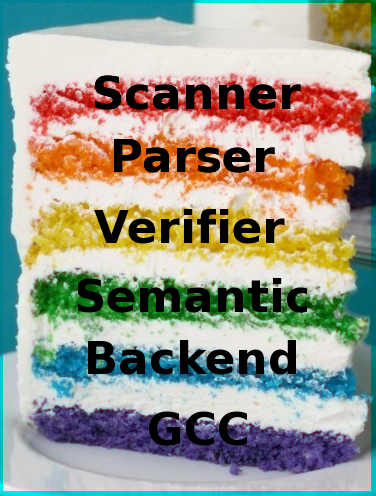
\includegraphics[width=40mm]{figures/layers.png}
\caption{A diagram showing the layers of \sys{}. The raw source code is
fed into the top of the cake and binary executables come out the bottom.
This image was manipulated by \sys{} using a Gaussian blur filter.}
\label{fig:layers}
\end{center}
\end{wrapfigure}

Our design incorporates six layers: the scanner, the parser, the verifier,
the semantic converter, the backend C generation, and C image manipulation
libraries (see Figure~\ref{fig:layers}). The compiler takes as input
a text file containing a valid \sys{} program and outputs a binary that
implements the program described by the input text.

The scanner generates as its output a one-dimensional list of
tokens (see Figure~\ref{fig:tokens}).

\begin{figure}
\begin{center}
\begin{tabular}{l l l l l l l}

    SEMI & LPAREN & RPAREN & LTCHAR & GTCHAR & LBRKT & RBRKT \\
    LBRACE & RBRACE COLON & COMMA & FSLASH & CONVOP & PIPE \\
    ATSYM & UMINUS & UPLUS & ASSIGN & DEFINE & OREQUAL & IMAGET \\
    KERNELT & CALCT & CHANNELT & UINT8T & UINT16T & UINT32T & INT8T \\
    INT16T & INT32T & ANGLET & IMGREAD & IMGWRITE & LITSTR & CSTR \\
    INTEGER & ID & EOF \\

\end{tabular}
\caption{A comprehensive list of tokens produced by the lexical analysis
(scanner).}
\end{center}
\label{fig:tokens}
\end{figure}

The parser reads this token list and uses our context-free grammar to generate
an abstract syntax tree. The parser is not strict about which nodes have
which children, or whether or not it is meaningful to have the current
structure: rather it just blindly assembles the tree. The abstract syntax tree
has the nodes described in Figure~\ref{fig:astnodes}.

\begin{figure}
\begin{center}
\begin{tabular}{l | l}
{\bf Node} & {\bf Description} \\
\hline \\
stmt & Statement \\
vdecl & Variable Declaration \\
expr & Expression \\
matrix & Calc matrix \\
bareint & Integer \\
kerncalc & Kernel calculation \\
chanref & Image channel reference \\
libfunc & \sys{} library function \\
assign\_op & Assignment operation \\
atom & Atomic type
\end{tabular}
\caption{A list of abstract syntax tree nodes.}
\label{fig:astnodes}
\end{center}
\end{figure}

The verifier accepts as input an abstract syntax tree. It traverses the
tree and checks that nodes are arranged in meaningful ways. While it
traverses, it also builds up an environment that keeps track of all
variables defined, along with their identifier name and type. If the
verifier accepts the AST, it will return as output the cumulative
environment that contains the identifiers and their types.

The semantic converter takes in a verified abstract syntax tree and also the
list of variables generated by the verifier. It then maps each node or
configuration of nodes to a corresponding Semantic AST node that
corresponds more directly with the eventual C code that must be generated.
The output of this layer is a semantically checked abstract syntax tree
(SAST). The semantic converter also supplements the environment information
inherited from the verifier with additional information not related to
verification, such the largest referenced command-line argument.

% TODO: Mapping of AST -> SAST ??

The backend takes as input the SAST and the supplemented environment
information. It then converts this into a meaningful C++ program source
file. This program can be submitted to GCC and compiled.

The final layer of \sys{} is the GCC compiler. The generated C source from
the backend is fed into the GCC compiler, which outputs a binary in
architecture-specific assembly language.

The lead developers for each layer of \sys{} are identified in
Figure~\ref{fig:leads}.


\begin{figure}
\begin{center}
\begin{tabular}{l | l}
{\bf Layer} & {\bf Lead Developer} \\
\hline \\
Unit Tests & Kevin and Yongxu \\
Scanner & Jeremy \\
Parser & Jeremy \\
Verifier & Jeremy \\
Semantic & Robert \\
Backend & Robert \\
GCC & Richard Stallman et al. \\
\end{tabular}
\caption{Who Did What: The lead developer of each layer.}
\end{center}
\label{fig:leads}
\end{figure}



    \chapter{Test Plan}
\label{chap:testplan}

Our unit test framework consists of pairs of identically named files in the \texttt{clam/tests/} directory.
Each pair consists of a CLAM program with extension \texttt{.clam} and an executable shell script
with extension \texttt{.test}. The CLAM file contains the code to be tested, while the shell script
specifies how to test that code: whether to compile and run or only compile, whether the test is supposed to fail,
what the expected output should look like, and what command line arguments to pass.
The \texttt{_buildup.sh} sets up the testing environment and defines common procedures such as
\texttt{compile-it} and \texttt{run-it}. Furthermore, \texttt{all.test} runs all tests in the directory,
tallies successes and failures and outputs a summary at the end.

Our testing is divided into four sections: syntax verification (section~\ref{testing:syntax}),
semantic/type verification (section~\ref{testing:semantic}),
CString verification (section~\ref{testing:cstrings}),
and functional output verification (section~\ref{testing:output}) which tests image processing results by comparison.

\section{Syntax Verification}
\label{testing:syntax}

Syntax verification testing is meant to confirm that the parser accepts all valid token strings,
and rejects all invalid ones as defined in our language reference manual.
We achieve this by inspecting \texttt{clam/parser.mly} and writing unit tests for
potentially problematic cases (many of the more straightforward rules were not deemed test-worthy).
All of these tests are only compiled and not executed. The testing process uncovered a number of errors
in matrix parsing and definition of kernel calculation lists.\\

\begin{itemize}

\item \texttt{matrix1.clam} tests that a simple matrix parses correctly, and should compile:
\lstinputlisting[language=CLAM]{../clam/tests/matrix1.clam}
(This originally failed because a scale factor was required, but now it is accepted.)

\item \texttt{matrix2.clam} tests that a matrix with scaling factor parses correctly, and should compile:
\lstinputlisting[language=CLAM]{../clam/tests/matrix2.clam}

\item \texttt{matrix3.clam} tests whether the parser catches ill-formed matrices, and should not compile:
\lstinputlisting[language=CLAM]{../clam/tests/matrix3.clam}
(This originally succeeded due to incorrect matrix parsing rules, but now it fails.)

\item \texttt{matrix4.clam} tests whether the parser catches another type of ill-formed matrix, and should also not compile:
\lstinputlisting[language=CLAM]{../clam/tests/matrix4.clam}
(This originally succeeded due to incorrect matrix parsing rules, but now it fails.)

\item \texttt{keyword-id.clam} tests whether the parser allows keywords to be identifiers, and should not compile:
\lstinputlisting[language=CLAM]{../clam/tests/keyword-id.clam}

\item \texttt{1calc-ker.clam} tests whether the parser allows \texttt{Kernel} definitions with only one \texttt{Calc}, and should compile:
\lstinputlisting[language=CLAM]{../clam/tests/keyword-id.clam}
(This originally failed because the original syntax caused reduce/reduce errors, so we changed both the parser and the test.
There was originally no \texttt{|} after the \texttt{=}.)

\item\texttt{string1.clam} checks that consecutive string literals are
  concatenated together into a single string literal. This should compile:
\lstinputlisting[language=CLAM]{../clam/tests/string1.clam}

\item \texttt{convoperand.clam} tests whether the \texttt{**} enforces a strict order of operands, and should not compile:
\lstinputlisting[language=CLAM]{../clam/tests/convoperand.clam}
(We only allow convolutions of the form \emph{channel-ref} \texttt{**} \emph{identifier}, in order to simplify
to translation into C code.)

\item \texttt{defcalc1.clam}, \texttt{defcalc2.clam}, and \texttt{defcalc3.clam} test various ways of declaring \texttt{Calc}s,
and all three should compile:
\lstinputlisting[language=CLAM]{../clam/tests/defcalc1.clam}
\lstinputlisting[language=CLAM]{../clam/tests/defcalc2.clam}
\lstinputlisting[language=CLAM]{../clam/tests/defcalc3.clam}

\item \texttt{rval-calc.clam}, \texttt{rval-matrix.clam}, \texttt{rval-chanref.clam}, \texttt{rval-conv.clam},
\texttt{rval-cstr.clam}, \texttt{rval-image.clam}, \texttt{rval-imgread.clam}, and \texttt{rval-kernel.clam}
test various "do nothing" statements consisting solely of r-values. Theses should all compile, though their
return values of the last line of each test are discarded so they do nothing:
\lstinputlisting[language=CLAM]{../clam/tests/rval-calc.clam}
\lstinputlisting[language=CLAM]{../clam/tests/rval-matrix.clam}
\lstinputlisting[language=CLAM]{../clam/tests/rval-chanref.clam}
\lstinputlisting[language=CLAM]{../clam/tests/rval-conv.clam}
\lstinputlisting[language=CLAM]{../clam/tests/rval-cstr.clam}
\lstinputlisting[language=CLAM]{../clam/tests/rval-image.clam}
\lstinputlisting[language=CLAM]{../clam/tests/rval-imgread.clam}
\lstinputlisting[language=CLAM]{../clam/tests/rval-kernel.clam}
(The parser accepted all of these, though most originally caused errors in the C translator
that had to be fixed (see "C Compiler Verification" below).)

\item \texttt{equality-trans.clam} checks that assignment expressions can be nested. This should compile:
\lstinputlisting[language=CLAM]{../clam/tests/equality-trans.clam}

\item \texttt{comment1.clam} checks that a program with only a comment (and zero statements) compiles. This should compile:
\lstinputlisting[language=CLAM]{../clam/tests/comment1.clam}

\end{itemize}

\section{Semantic Verification}
\label{testing:semantic}

Semantic verification testing is meant to confirm that the verifier accepts all valid parse trees,
and rejects all invalid ones according to the specifications of our language
(and according to what makes sense).
These tests depend on \texttt{clam/verifier.ml}, as well as \texttt{clam/environ.ml} and \texttt{envtypes.mli}. 
The testing process uncovered a number of errors in matrix verification (separate from syntax)
and the creation of default RGB Channels.\\

\begin{itemize}

\item\texttt{zerocalc1.clam} and \texttt{zerocalc2.clam} check that a matrix scaling-factor can
have a numerator of zero, but not a denominator of zero.
The former should certainly compile, while the latter should not:
\lstinputlisting[language=CLAM]{../clam/tests/zerocalc1.clam}
\lstinputlisting[language=CLAM]{../clam/tests/zerocalc2.clam}
(\texttt{zerocalc2.clam} originally passed verification, but that was fixed.)

\item\texttt{invalid1.clam} checks that undeclared identifiers are caught. This should not compile:
\lstinputlisting[language=CLAM]{../clam/tests/invalid1.clam}

\item\texttt{undefined1.clam} checks that an undefined Channel reference cannot be an r-value. This should not compile:
\lstinputlisting[language=CLAM]{../clam/tests/undefined1.clam}

\item\texttt{imgchannel1.clam} checks that an \texttt{Image} has default channels when read. This should compile:
\lstinputlisting[language=CLAM]{../clam/tests/imgchannel1.clam}

\item\texttt{imgchannel2.clam} checks that an undefined \texttt{Calc} cannot be applied to an \texttt{Image}. This should not compile:
\lstinputlisting[language=CLAM]{../clam/tests/imgchannel2.clam}

\item\texttt{imgchannel3.clam} checks that a \texttt{Calc} defined as a matrix cannot be applied to an \texttt{Image}. This should not compile:
\lstinputlisting[language=CLAM]{../clam/tests/imgchannel3.clam}

\item\texttt{imgchannel4.clam} checks that a \texttt{Calc} defined as a CString \emph{can} be applied to an \texttt{Image}. This should compile:
\lstinputlisting[language=CLAM]{../clam/tests/imgchannel4.clam}

\item\texttt{image-eq-image.clam} checks \texttt{=} assignment for images to images. This should compile:
\lstinputlisting[language=CLAM]{../clam/tests/image-eq-image.clam}

\item\texttt{image-oreq-image.clam} checks \texttt{|=} assignment for images to images. This is not supported and doesn't compile:
\lstinputlisting[language=CLAM]{../clam/tests/image-oreq-image.clam}

\item\texttt{image-defeq.clam} checks \texttt{:=} assignment for images. This is not supported and doesn't compile:
\lstinputlisting[language=CLAM]{../clam/tests/image-defeq.clam}

\item\texttt{imgread-bad.clam} checks that l-value identifiers have to be declared first. This shouldn't compile:
\lstinputlisting[language=CLAM]{../clam/tests/imgread-bad.clam}

\item\texttt{imgread-bad2.clam} checks that \texttt{imgread} must be called with only one argument. This shouldn't compile:
\lstinputlisting[language=CLAM]{../clam/tests/imgread-bad2.clam}

\item\texttt{imgread-bad3.clam} checks that \texttt{imgread} can only be called with a literal string or integer. This shouldn't compile:
\lstinputlisting[language=CLAM]{../clam/tests/imgread-bad3.clam}

\item\texttt{imgread.clam} checks that \texttt{imgread} can actually called with a correct argument. This should compile:
\lstinputlisting[language=CLAM]{../clam/tests/imgread-bad.clam}

\item\texttt{imgwrite-bad1.clam} checks that \texttt{imgwrite} can't be called with incorrect number and type of arguments. This shouldn't compile:
\lstinputlisting[language=CLAM]{../clam/tests/imgwrite-bad1.clam}

\item\texttt{defchannels.clam} checks that the default RGB Channels don't exist for a declared-but-not-read \texttt{Image}. This shouldn't compile:
\lstinputlisting[language=CLAM]{../clam/tests/defchannels.clam}
(Allowing default RGB channels for an unread \texttt{Image} is problematic because CLAM
does not allow explicit manipulation of Channel \emph{size}.)

\item\texttt{imgwrite-norgb.clam} checks that a declared-but-not-read \texttt{Image} without RGB channels
(and more importantly, without a \emph{size}) cannot be written. This shouldn't compile:
\lstinputlisting[language=CLAM]{../clam/tests/imgwrite-norgb.clam}

\item\texttt{sizediff.clam} checks that the default Channels from \texttt{Image}s of different sizes
cannot be assigned to each other, because all Channels of an \texttt{Image} should have the same size. This shouldn't compile:
\lstinputlisting[language=CLAM]{../clam/tests/sizediff.clam}

\item\texttt{at-channel.clam} checks that transient \texttt{Calc}s marked with \texttt{@} in a \texttt{Kernel}
do not result in Channels after a convolution. This shouldn't compile:
\lstinputlisting[language=CLAM]{../clam/tests/at-channel.clam}

\item\texttt{addker.clam} checks a \texttt{Kernel} can be appended to another \texttt{Kernel} using \texttt{|=}. This should compile:
\lstinputlisting[language=CLAM]{../clam/tests/addker.clam}

\item\texttt{DefEq.clam} checks that \texttt{=} cannot be used to define a \texttt{Calc}. This should not compile:
\lstinputlisting[language=CLAM]{../clam/tests/DefEq.clam}

\item\texttt{ckernel.clam} checks that \texttt{Kernel}s must be defined using \texttt{Calc} \emph{identifiers}
and not anonymous \texttt{Calc} expressions. This should not compile:
\lstinputlisting[language=CLAM]{../clam/tests/ckernel.clam}

\item\texttt{cimage.clam} checks that \texttt{Image}s cannot be defined using \texttt{Calc} expressions. This should not compile:
\lstinputlisting[language=CLAM]{../clam/tests/cimage.clam}

\end{itemize}

\section{CString Verification}
\label{testing:cstrings}

CString verification testing checks that invalid CStrings are caught before being passed to GCC, where they
could cause fatal errors. Of course, it is impossible to catch \emph{all} possible errors without
building an understanding of C syntax directly into CLAM, so we are satisfied with catching common
mistakes and rely on the user and GCC error messages for everything else. (For example, a CString of the form \texttt{\#[while(1)]\#},
while certainly disruptive, will compile and it is the user's fault that the program stalls.)
For each possible issue that we \emph{did} choose to catch, we wrote unit tests to confirm that they were caught.
Catching of invalid CStrings is done entirely in \texttt{clam/scanner.mll}. Testing reveals errors
in parentheses matching, which were promptly corrected.\\

\begin{itemize}

\item\texttt{cstring1.clam} checks that C preprocessor cannot be used in a CString. This should not compile:
\lstinputlisting[language=CLAM]{../clam/tests/cstring1.clam}

\item\texttt{cstring2.clam} checks that C comments cannot be used in a CString. This should not compile:
\lstinputlisting[language=CLAM]{../clam/tests/cstring2.clam}

\item\texttt{cstring3.clam} checks that empty CStrings are OK, and just result in an empty statement. This should compile:
\lstinputlisting[language=CLAM]{../clam/tests/cstring3.clam}

\item\texttt{cstring4.clam} checks that library calls in a CString must be closed. This should not compile:
\lstinputlisting[language=CLAM]{../clam/tests/cstring4.clam}
(This originally did compile because the scanner didn't record nesting-level properly. It was fixed.)

\item\texttt{cstring5.clam} checks that parentheses in a CString must be matched. This should not compile:
\lstinputlisting[language=CLAM]{../clam/tests/cstring5.clam}
(This originally did compile because the scanner didn't record nesting-level properly. It was fixed.)

\item\texttt{cstring6.clam} is a sanity check that "normal" CStrings do in fact work. This should obviously compile:
\lstinputlisting[language=CLAM]{../clam/tests/cstring6.clam}

\end{itemize}

\section{C Compiler Verification}
\label{testing:ccompiler}

A few of the above tests, which originally compiled, began failing once the C backend was hooked up.
The most common errors were with C syntax and memory allocation.
While we didn't write tests specifically targeted at the C backend,
the tests we wrote for other parts of the architecture also helped us identify problems in the C translator. 

\section{Image Processing Verification}
\label{testing:output}

These are comprehensive tests, consisting of full-fledged programs that actually
read, manipulate and write images. While the testing framework provides image-comparison functionality,
most verification here is actually done with the naked eye.\\

\begin{itemize}

\item\texttt{imgcopy.clam} copies an image. This should compile, run, and copy an image:
\lstinputlisting[language=CLAM]{../clam/tests/imgcopy.clam}

\item\texttt{sobel.clam} applies the Sobel operation to an image. This should compile, run, and output
a map of the luminosity gradient:
\lstinputlisting[language=CLAM]{../clam/tests/sobel.clam}

\end{itemize}



    \chapter{Lessons Learned}


    \appendix
    \chapter{Complete Code Reference}
\label{chap:coderef}
The \sys{} programming language was implemented in OCaml. It uses the
C/C++ programming languages as backend targets, and invokes the \texttt{g++}
compiler on the \sys{} compilation output to produce a final binary. The
final binary is statically linked against a \sys{} implementation library,
\texttt{clam.a}, which contains the low-level image manipulation functions. Additionally,
\sys{} leveraged several OCaml functions from the \emph{extlib}~\cite{extlib:googlecode}
project, and a stand-alone image reader~\cite{stbimage:read} and writer~\cite{stbimage:write}
library written by Sean Barrett. Code listings of the \sys{} compiler and \sys{} implementation library
as well as the subset of \emph{extlib} used by \sys{} follow:

\clearpage
\section{\sys{} Compiler}
\lstinputlisting[language=Ocaml]{../clam/clam.ml} \clearpage
\lstinputlisting[language=Ocaml]{../clam/ast.mli} \clearpage
\lstinputlisting[language=Ocaml]{../clam/backend.ml} \clearpage
\lstinputlisting[language=Ocaml]{../clam/clamsys.ml} \clearpage
\lstinputlisting[language=Ocaml]{../clam/environ.ml} \clearpage
\lstinputlisting[language=Ocaml]{../clam/envtypes.mli} \clearpage
\lstinputlisting[language=Ocaml]{../clam/parseutil.ml} \clearpage
\lstinputlisting[language=Ocaml]{../clam/parser.mly} \clearpage
\lstinputlisting[language=Ocaml]{../clam/printer.ml} \clearpage
\lstinputlisting[language=Ocaml]{../clam/sast.mli} \clearpage
\lstinputlisting[language=Ocaml]{../clam/scanner.mll} \clearpage
\lstinputlisting[language=Ocaml]{../clam/semantic.ml} \clearpage
\lstinputlisting[language=Ocaml]{../clam/verifier.ml} \clearpage

\subsection{Subset of \emph{extlib} Used by \sys{}}
\sys{} compiled the following source files from the \texttt{extlib}~\cite{extlib:googlecode}
project. Their full source is omitted for brevity -- see the project website.
\begin{itemize}
  \item{\texttt{enum.ml}}
  \item{\texttt{enum.mli}}
  \item{\texttt{extString.ml}}
  \item{\texttt{extString.mli}}
  \item{\texttt{std.ml}}
  \item{\texttt{std.mli}}
\end{itemize}
\comment{
  \lstinputlisting[language=Ocaml]{../clam/extlib/enum.ml} \clearpage
  \lstinputlisting[language=Ocaml]{../clam/extlib/enum.mli} \clearpage
  \lstinputlisting[language=Ocaml]{../clam/extlib/extString.ml} \clearpage
  \lstinputlisting[language=Ocaml]{../clam/extlib/extString.mli} \clearpage
  \lstinputlisting[language=Ocaml]{../clam/extlib/std.ml} \clearpage
  \lstinputlisting[language=Ocaml]{../clam/extlib/std.mli} \clearpage
} % END-COMMENT

\section{\sys{} Implementation Library (\texttt{clam.a})}
\definecolor{cstyleDarkRed}{rgb}{0.65, 0.08, 0.0}
\definecolor{cstyleDarkBlue}{rgb}{0.0, 0.08, 0.65}
\definecolor{cstyleGrey}{rgb}{0.55, 0.55, 0.55}
\lstset{
    keywordstyle={\color{cstyleDarkRed}\bfseries},
    commentstyle={\color{cstyleGrey}\bfseries},
    %directivestyle={\color{cstyleDarkBlue}},
    sensitive=true,
    showstringspaces=false,
    showspaces=false,
    showtabs=false,
    numbers=left,
    frame=single,
    breaklines=true,
    basicstyle=\ttfamily\scriptsize,
}
%\subsection{\sys{} C Source}
\lstinputlisting[language=C]{../clam/libstb/clam.h} \clearpage
\lstinputlisting[language=C]{../clam/libstb/clam.c} \clearpage
%\subsection{\texttt{stb\_image} Source}
%\lstinputlisting[language=C]{../clam/libstb/stb-image-read.c} \clearpage
%\lstinputlisting[language=C]{../clam/libstb/stb-image-write.c} \clearpage

\section{Unit Test Framework}
Our unit testing framework was built on two custom shell scripts that provided
a framework to compile a test program, determine success/failure of compilation,
compare image outputs and report overall success or failure of the test.
The framework simply runs all shell scripts in the \emph{test} directory and
reports the success/failure of each one (with a summary of failures at the end).
The \texttt{_buildup.sh}, \texttt{_breakdown.sh}, and \texttt{all.test} scripts are
reported here, followed by all of the tests and a sample run of the
\texttt{all.test} script.
\vskip -4mm

\vskip -4mm
\subsection*{_buildup.sh}
\vskip -2mm
\lstinputlisting[language=bash]{../clam/tests/build-up-script-link.sh} \clearpage
\subsection*{_breakdown.sh}
\lstinputlisting[language=bash]{../clam/tests/breakdown-script-link.sh}
\subsection*{all.test}
\lstinputlisting[language=bash]{../clam/tests/all.test} \clearpage
% all the tests 
\subsection*{The tests (shell script followed by \sys{} source)}
\subsection*{Unit Test: 1calc-ker}
\lstinputlisting[language=bash]{../clam/tests/1calc-ker.test}
\lstinputlisting[language=bash]{../clam/tests/1calc-ker.clam} \clearpage
\subsection*{Unit Test: DefEq}
\lstinputlisting[language=bash]{../clam/tests/DefEq.test}
\lstinputlisting[language=bash]{../clam/tests/DefEq.clam} \clearpage
\subsection*{Unit Test: addker}
\lstinputlisting[language=bash]{../clam/tests/addker.test}
\lstinputlisting[language=bash]{../clam/tests/addker.clam} \clearpage
\subsection*{Unit Test: at-channel}
\lstinputlisting[language=bash]{../clam/tests/at-channel.test}
\lstinputlisting[language=bash]{../clam/tests/at-channel.clam} \clearpage
\subsection*{Unit Test: cimage}
\lstinputlisting[language=bash]{../clam/tests/cimage.test}
\lstinputlisting[language=bash]{../clam/tests/cimage.clam} \clearpage
\subsection*{Unit Test: ckernel}
\lstinputlisting[language=bash]{../clam/tests/ckernel.test}
\lstinputlisting[language=bash]{../clam/tests/ckernel.clam} \clearpage
\subsection*{Unit Test: comment1}
\lstinputlisting[language=bash]{../clam/tests/comment1.test}
\lstinputlisting[language=bash]{../clam/tests/comment1.clam} \clearpage
\subsection*{Unit Test: convoperand}
\lstinputlisting[language=bash]{../clam/tests/convoperand.test}
\lstinputlisting[language=bash]{../clam/tests/convoperand.clam} \clearpage
\subsection*{Unit Test: cstring1}
\lstinputlisting[language=bash]{../clam/tests/cstring1.test}
\lstinputlisting[language=bash]{../clam/tests/cstring1.clam} \clearpage
\subsection*{Unit Test: cstring2}
\lstinputlisting[language=bash]{../clam/tests/cstring2.test}
\lstinputlisting[language=bash]{../clam/tests/cstring2.clam} \clearpage
\subsection*{Unit Test: cstring3}
\lstinputlisting[language=bash]{../clam/tests/cstring3.test}
\lstinputlisting[language=bash]{../clam/tests/cstring3.clam} \clearpage
\subsection*{Unit Test: cstring4}
\lstinputlisting[language=bash]{../clam/tests/cstring4.test}
\lstinputlisting[language=bash]{../clam/tests/cstring4.clam} \clearpage
\subsection*{Unit Test: cstring5}
\lstinputlisting[language=bash]{../clam/tests/cstring5.test}
\lstinputlisting[language=bash]{../clam/tests/cstring5.clam} \clearpage
\subsection*{Unit Test: cstring6}
\lstinputlisting[language=bash]{../clam/tests/cstring6.test}
\lstinputlisting[language=bash]{../clam/tests/cstring6.clam} \clearpage
\subsection*{Unit Test: defcalc1}
\lstinputlisting[language=bash]{../clam/tests/defcalc1.test}
\lstinputlisting[language=bash]{../clam/tests/defcalc1.clam} \clearpage
\subsection*{Unit Test: defcalc2}
\lstinputlisting[language=bash]{../clam/tests/defcalc2.test}
\lstinputlisting[language=bash]{../clam/tests/defcalc2.clam} \clearpage
\subsection*{Unit Test: defcalc3}
\lstinputlisting[language=bash]{../clam/tests/defcalc3.test}
\lstinputlisting[language=bash]{../clam/tests/defcalc3.clam} \clearpage
\subsection*{Unit Test: defchannels}
\lstinputlisting[language=bash]{../clam/tests/defchannels.test}
\lstinputlisting[language=bash]{../clam/tests/defchannels.clam} \clearpage
\subsection*{Unit Test: equality-trans}
\lstinputlisting[language=bash]{../clam/tests/equality-trans.test}
\lstinputlisting[language=bash]{../clam/tests/equality-trans.clam} \clearpage
\subsection*{Unit Test: id-overlap}
\lstinputlisting[language=bash]{../clam/tests/id-overlap.test}
\lstinputlisting[language=bash]{../clam/tests/id-overlap.clam} \clearpage
\subsection*{Unit Test: image-defeq}
\lstinputlisting[language=bash]{../clam/tests/image-defeq.test}
\lstinputlisting[language=bash]{../clam/tests/image-defeq.clam} \clearpage
\subsection*{Unit Test: image-eq-image}
\lstinputlisting[language=bash]{../clam/tests/image-eq-image.test}
\lstinputlisting[language=bash]{../clam/tests/image-eq-image.clam} \clearpage
\subsection*{Unit Test: image-oreq-image}
\lstinputlisting[language=bash]{../clam/tests/image-oreq-image.test}
\lstinputlisting[language=bash]{../clam/tests/image-oreq-image.clam} \clearpage
\subsection*{Unit Test: imgchannel1}
\lstinputlisting[language=bash]{../clam/tests/imgchannel1.test}
\lstinputlisting[language=bash]{../clam/tests/imgchannel1.clam} \clearpage
\subsection*{Unit Test: imgchannel2}
\lstinputlisting[language=bash]{../clam/tests/imgchannel2.test}
\lstinputlisting[language=bash]{../clam/tests/imgchannel2.clam} \clearpage
\subsection*{Unit Test: imgchannel3}
\lstinputlisting[language=bash]{../clam/tests/imgchannel3.test}
\lstinputlisting[language=bash]{../clam/tests/imgchannel3.clam} \clearpage
\subsection*{Unit Test: imgchannel4}
\lstinputlisting[language=bash]{../clam/tests/imgchannel4.test}
\lstinputlisting[language=bash]{../clam/tests/imgchannel4.clam} \clearpage
\subsection*{Unit Test: imgcopy}
\lstinputlisting[language=bash]{../clam/tests/imgcopy.test}
\lstinputlisting[language=bash]{../clam/tests/imgcopy.clam} \clearpage
\subsection*{Unit Test: imgread}
\lstinputlisting[language=bash]{../clam/tests/imgread.test}
\lstinputlisting[language=bash]{../clam/tests/imgread.clam} \clearpage
\subsection*{Unit Test: imgread-bad}
\lstinputlisting[language=bash]{../clam/tests/imgread-bad.test}
\lstinputlisting[language=bash]{../clam/tests/imgread-bad.clam} \clearpage
\subsection*{Unit Test: imgread-bad2}
\lstinputlisting[language=bash]{../clam/tests/imgread-bad2.test}
\lstinputlisting[language=bash]{../clam/tests/imgread-bad2.clam} \clearpage
\subsection*{Unit Test: imgread-bad3}
\lstinputlisting[language=bash]{../clam/tests/imgread-bad3.test}
\lstinputlisting[language=bash]{../clam/tests/imgread-bad3.clam} \clearpage
\subsection*{Unit Test: imgwrite-bad1}
\lstinputlisting[language=bash]{../clam/tests/imgwrite-bad1.test}
\lstinputlisting[language=bash]{../clam/tests/imgwrite-bad1.clam} \clearpage
\subsection*{Unit Test: imgwrite-norgb}
\lstinputlisting[language=bash]{../clam/tests/imgwrite-norgb.test}
\lstinputlisting[language=bash]{../clam/tests/imgwrite-norgb.clam} \clearpage
\subsection*{Unit Test: invalid1}
\lstinputlisting[language=bash]{../clam/tests/invalid1.test}
\lstinputlisting[language=bash]{../clam/tests/invalid1.clam} \clearpage
\subsection*{Unit Test: keyword-id}
\lstinputlisting[language=bash]{../clam/tests/keyword-id.test}
\lstinputlisting[language=bash]{../clam/tests/keyword-id.clam} \clearpage
\subsection*{Unit Test: matrix1}
\lstinputlisting[language=bash]{../clam/tests/matrix1.test}
\lstinputlisting[language=bash]{../clam/tests/matrix1.clam} \clearpage
\subsection*{Unit Test: matrix2}
\lstinputlisting[language=bash]{../clam/tests/matrix2.test}
\lstinputlisting[language=bash]{../clam/tests/matrix2.clam} \clearpage
\subsection*{Unit Test: matrix3}
\lstinputlisting[language=bash]{../clam/tests/matrix3.test}
\lstinputlisting[language=bash]{../clam/tests/matrix3.clam} \clearpage
\subsection*{Unit Test: matrix4}
\lstinputlisting[language=bash]{../clam/tests/matrix4.test}
\lstinputlisting[language=bash]{../clam/tests/matrix4.clam} \clearpage
\subsection*{Unit Test: rval-calc}
\lstinputlisting[language=bash]{../clam/tests/rval-calc.test}
\lstinputlisting[language=bash]{../clam/tests/rval-calc.clam} \clearpage
\subsection*{Unit Test: rval-chanref}
\lstinputlisting[language=bash]{../clam/tests/rval-chanref.test}
\lstinputlisting[language=bash]{../clam/tests/rval-chanref.clam} \clearpage
\subsection*{Unit Test: rval-conv}
\lstinputlisting[language=bash]{../clam/tests/rval-conv.test}
\lstinputlisting[language=bash]{../clam/tests/rval-conv.clam} \clearpage
\subsection*{Unit Test: rval-cstr}
\lstinputlisting[language=bash]{../clam/tests/rval-cstr.test}
\lstinputlisting[language=bash]{../clam/tests/rval-cstr.clam} \clearpage
\subsection*{Unit Test: rval-image}
\lstinputlisting[language=bash]{../clam/tests/rval-image.test}
\lstinputlisting[language=bash]{../clam/tests/rval-image.clam} \clearpage
\subsection*{Unit Test: rval-imgread}
\lstinputlisting[language=bash]{../clam/tests/rval-imgread.test}
\lstinputlisting[language=bash]{../clam/tests/rval-imgread.clam} \clearpage
\subsection*{Unit Test: rval-kernel}
\lstinputlisting[language=bash]{../clam/tests/rval-kernel.test}
\lstinputlisting[language=bash]{../clam/tests/rval-kernel.clam} \clearpage
\subsection*{Unit Test: rval-matrix}
\lstinputlisting[language=bash]{../clam/tests/rval-matrix.test}
\lstinputlisting[language=bash]{../clam/tests/rval-matrix.clam} \clearpage
\subsection*{Unit Test: sizediff}
\lstinputlisting[language=bash]{../clam/tests/sizediff.test}
\lstinputlisting[language=bash]{../clam/tests/sizediff.clam} \clearpage
\subsection*{Unit Test: sobel}
\lstinputlisting[language=bash]{../clam/tests/sobel.test}
\lstinputlisting[language=bash]{../clam/tests/sobel.clam} \clearpage
\subsection*{Unit Test: undefined1}
\lstinputlisting[language=bash]{../clam/tests/undefined1.test}
\lstinputlisting[language=bash]{../clam/tests/undefined1.clam} \clearpage
\subsection*{Unit Test: zerocalc1}
\lstinputlisting[language=bash]{../clam/tests/zerocalc1.test}
\lstinputlisting[language=bash]{../clam/tests/zerocalc1.clam} \clearpage
\subsection*{Unit Test: zerocalc2}
\lstinputlisting[language=bash]{../clam/tests/zerocalc2.test}
\lstinputlisting[language=bash]{../clam/tests/zerocalc2.clam} \clearpage

\chapter{Project Version Control History}
\label{chap:vcshistory}
The \sys{} project used \texttt{git}~\cite{git:website} as its version control system.
Here we provide the output of the \texttt{git-shortlog} program with \emph{Merge}
commits filtered out, followed by a more complete revision control history.

\input{clam.gitlog}

    \clearpage
  \fi
  {
    \balance
    \bibliographystyle{abbrv}
    \bibliography{clam}
  }
\fi

\end{document}


    \clearpage
  \fi
  {
    \balance
    \bibliographystyle{abbrv}
    \bibliography{paper}
  }
\fi

\end{document}
